\subsection{Mockups}
\label{subsec:mockups_quejoso}

Los mockups presentados en esta sección representan el diseño visual de alto nivel de la interfaz de usuario del Módulo del Quejoso, desarrollada con el framework Angular. Cada pantalla ha sido diseñada siguiendo los lineamientos de la Defensoría de los Derechos Politécnicos, priorizando la accesibilidad, la claridad informativa y la guía al usuario a lo largo de los distintos flujos funcionales descritos en los Casos de Uso. Las vistas se organizan en el orden natural de navegación del quejoso: desde el punto de entrada al portal, pasando por el registro y autenticación, hasta la gestión completa de expedientes y propuestas de conciliación.

% ---- MQ-01 ----
\subsubsection{MQ-01: Pantalla de Inicio}

Es el punto de acceso principal para la comunidad politécnica. Presenta una interfaz limpia con tres acciones principales: presentar una nueva queja, dar seguimiento a un trámite existente como invitado, o iniciar sesión. Incluye elementos informativos sobre los derechos y el propósito de la Defensoría.

\begin{figure}[H]
    \centering
    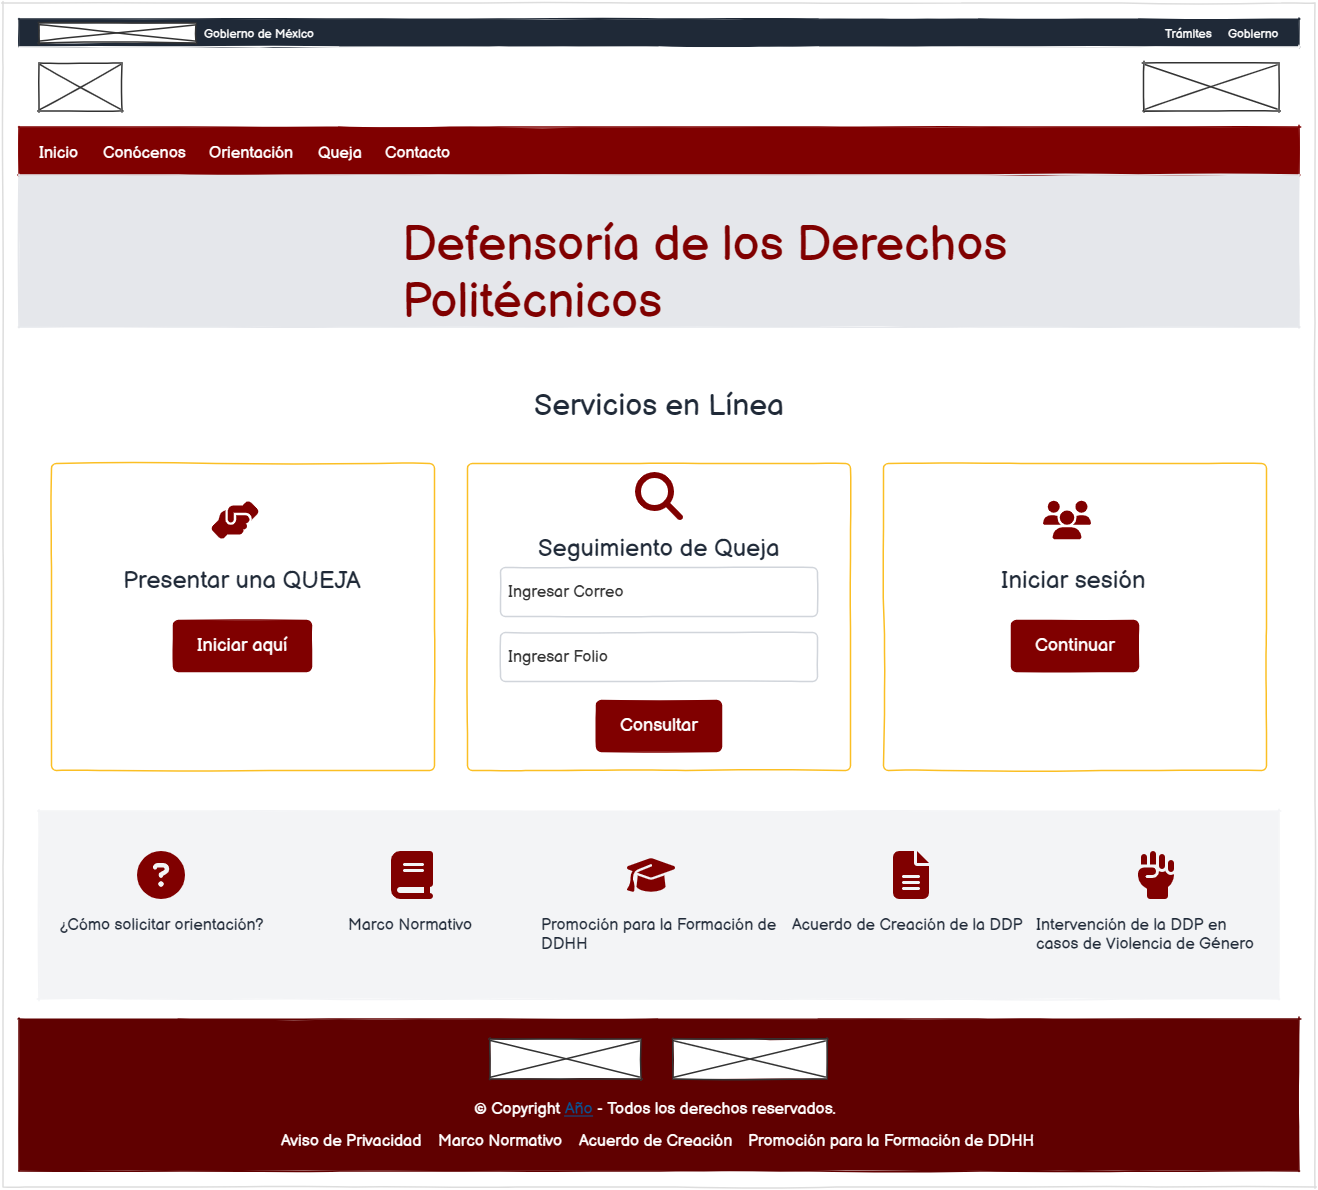
\includegraphics[width=0.80\textwidth, height=0.70\textheight, keepaspectratio]{imagenes/quejoso/Mockups/MQ-01_PantallaInicio.png}
    \caption{Mockup MQ-01: Pantalla de Inicio del Portal}
    \label{fig:mq01_pantalla_inicio}
\end{figure}

% ---- MQ-02 ----
\subsubsection{MQ-02: Formulario de Registro de Queja}

Interfaz diseñada para la captura de información de una queja. Se divide en secciones lógicas: datos personales del quejoso, narrativa detallada de los hechos y un área de carga de archivos multimedia para las evidencias. Utiliza validaciones para asegurar que los campos obligatorios sean completados correctamente.

\begin{figure}[H]
    \centering
    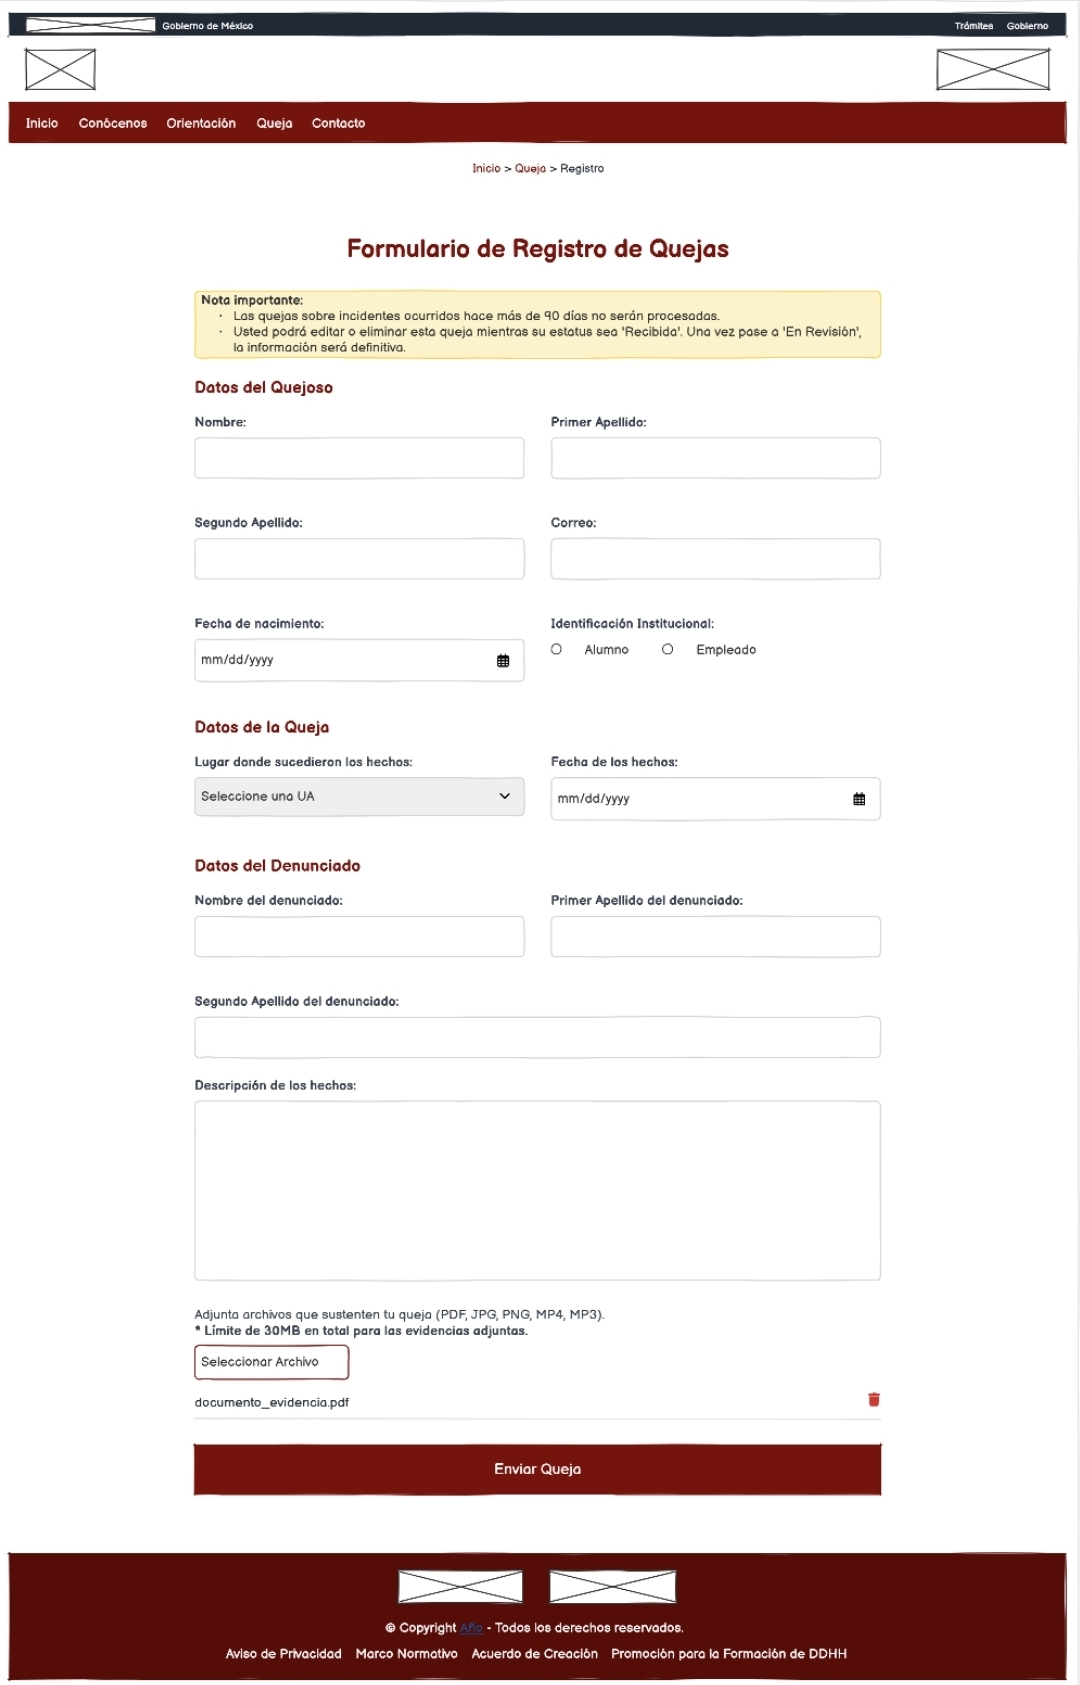
\includegraphics[width=0.80\textwidth, height=0.70\textheight, keepaspectratio]{imagenes/quejoso/Mockups/MQ-02_FormularioRegistro.jpg}
    \caption{Mockup MQ-02: Formulario de Registro de Queja}
    \label{fig:mq02_formulario_registro}
\end{figure}

% ---- MQ-03 ----
\subsubsection{MQ-03: Ventana de Datos del Tutor}

Componente modal que se activa automáticamente cuando el sistema detecta que el quejoso es menor de edad basándose en su fecha de nacimiento. Solicita los datos de contacto y parentesco de un adulto responsable para proceder con la validez jurídica del trámite.

\begin{figure}[H]
    \centering
    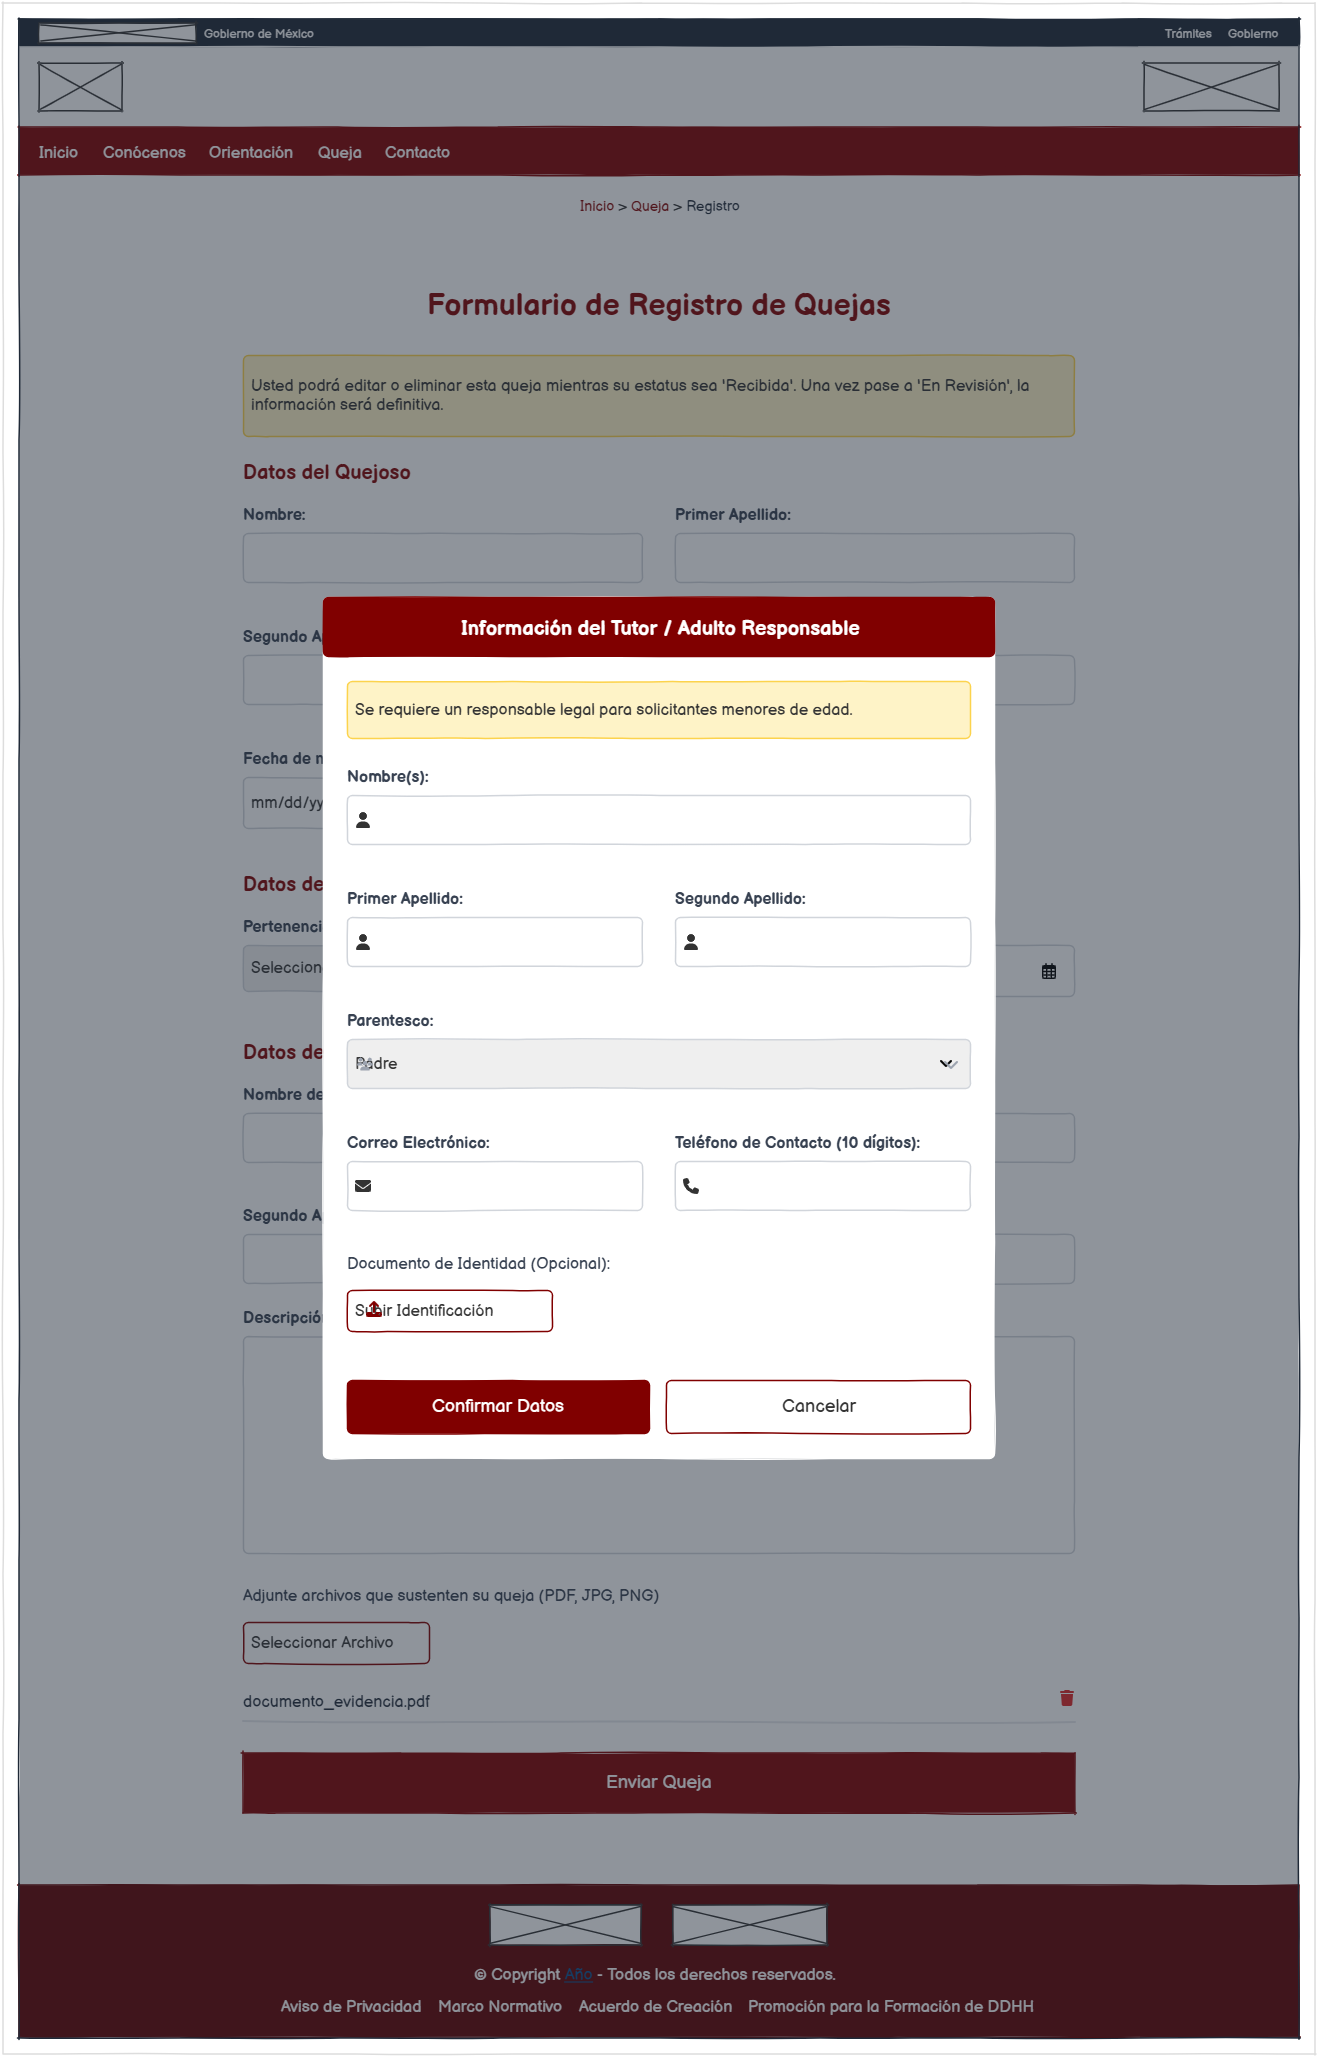
\includegraphics[width=0.80\textwidth, height=0.70\textheight, keepaspectratio]{imagenes/quejoso/Mockups/MQ-03_VentanaTutor.png}
    \caption{Mockup MQ-03: Ventana de Datos del Tutor}
    \label{fig:mq03_ventana_tutor}
\end{figure}

% ---- MQ-04 ----
\subsubsection{MQ-04: Pantalla de Éxito y Folio}

Vista de confirmación tras el envío exitoso de la queja. Muestra el folio único de seguimiento generado por el sistema. Ofrece al usuario dos vías de acción inmediata: descargar el acuse de recibo en formato PDF o proceder a la configuración de una cuenta para seguimiento detallado.

\begin{figure}[H]
    \centering
    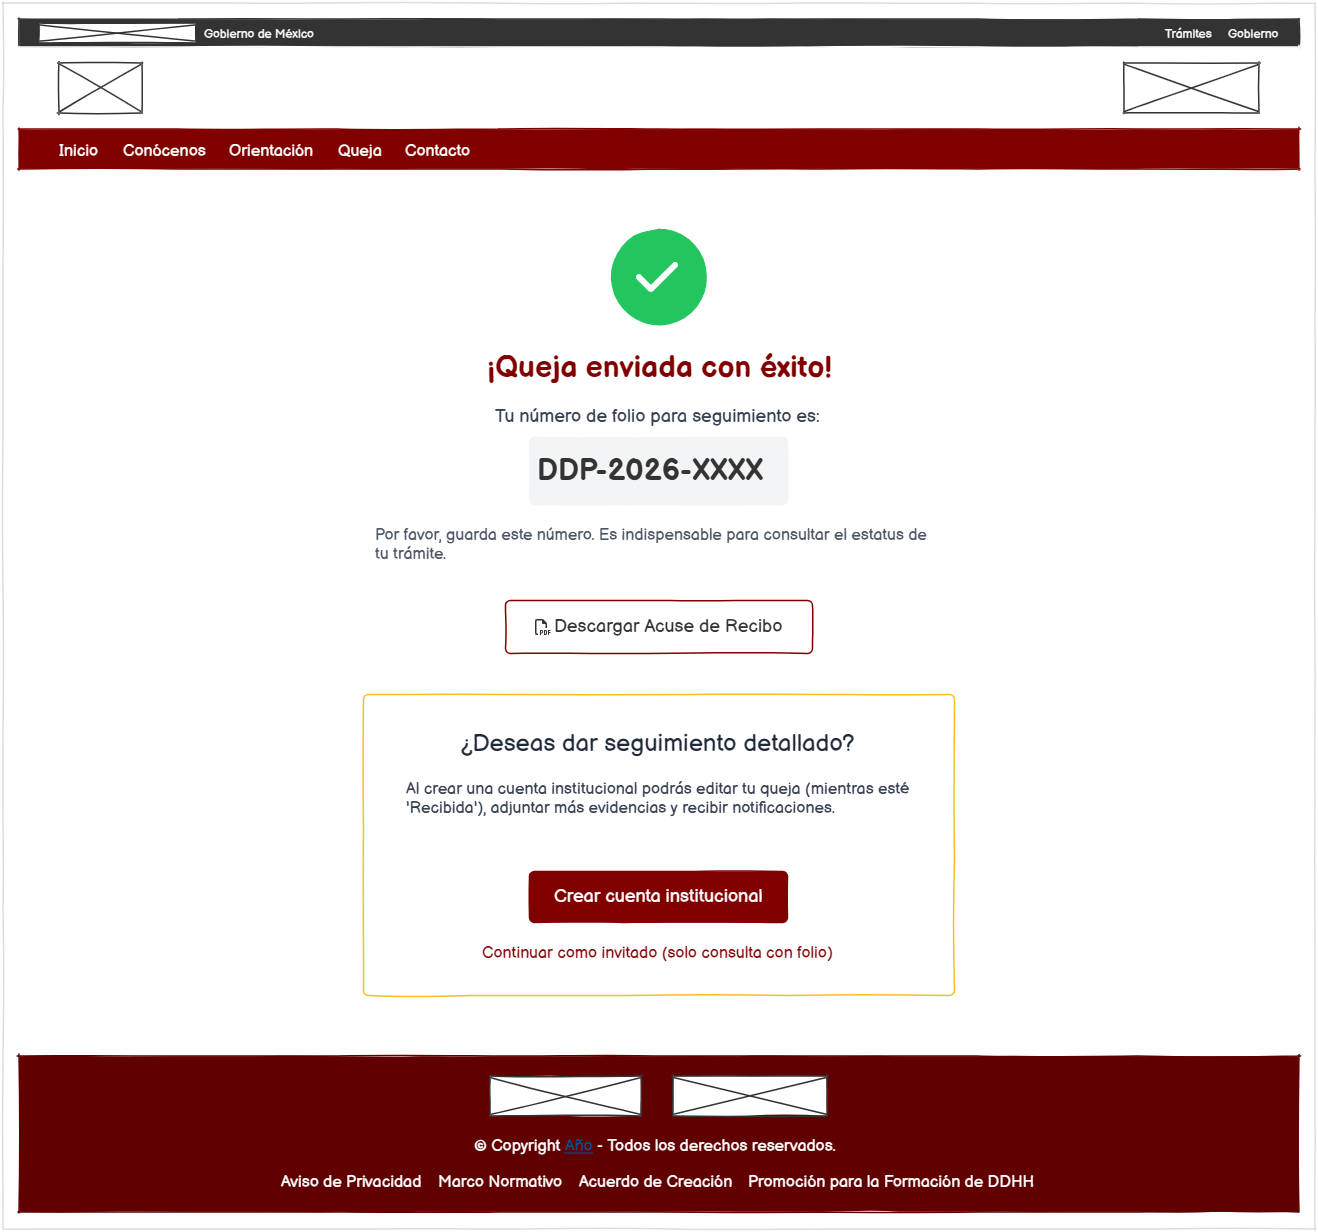
\includegraphics[width=0.80\textwidth, height=0.70\textheight, keepaspectratio]{imagenes/quejoso/Mockups/MQ-04_ExitoFolio.png}
    \caption{Mockup MQ-04: Pantalla de Éxito con Folio Generado}
    \label{fig:mq04_exito_folio}
\end{figure}

% ---- MQ-05 ----
\subsubsection{MQ-05: Configuración de Cuenta}

Pantalla dedicada a la transición de usuario invitado a registrado. Permite al quejoso establecer una contraseña de acceso segura vinculada al correo proporcionado en el registro. Es el paso previo para habilitar el acceso al Dashboard institucional.

\begin{figure}[H]
    \centering
    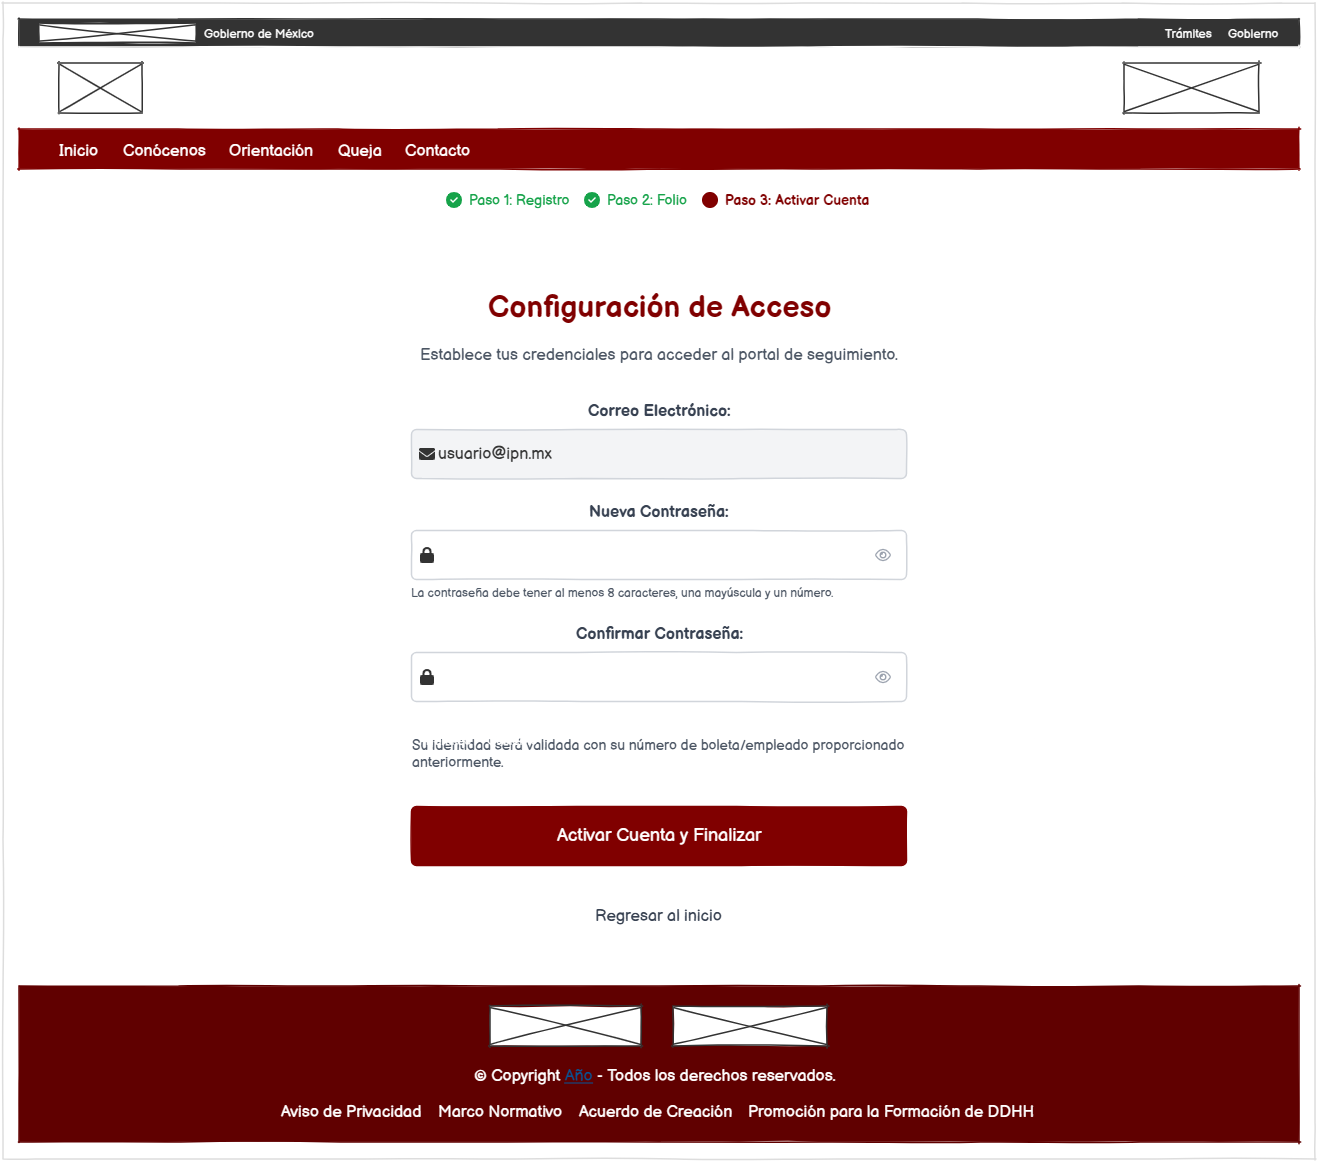
\includegraphics[width=0.80\textwidth, height=0.70\textheight, keepaspectratio]{imagenes/quejoso/Mockups/MQ-05_ConfiguracionCuenta.png}
    \caption{Mockup MQ-05: Configuración de Cuenta de Seguimiento}
    \label{fig:mq05_configuracion_cuenta}
\end{figure}

% ---- MQ-06 ----
\subsubsection{MQ-06: Seguimiento sin Cuenta}

Interfaz simplificada para el seguimiento de trámites sin necesidad de iniciar sesión. Permite a los usuarios que optaron por no crear una cuenta verificar el estatus de su trámite ingresando únicamente el folio y el correo electrónico asociado. Ofrece una vista resumida del estado actual del expediente, proporcionando información clave como la etapa administrativa y evidencias.

\begin{figure}[H]
    \centering
    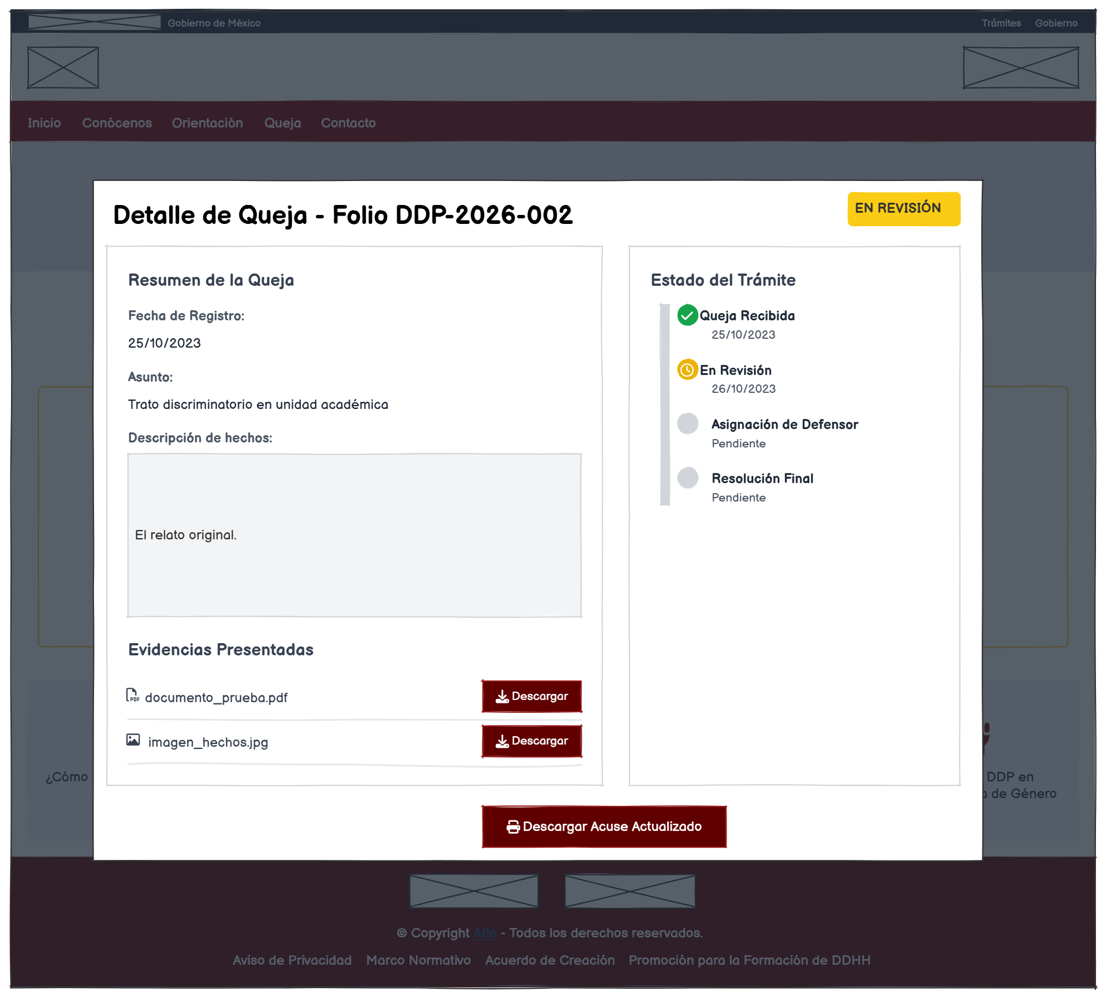
\includegraphics[width=0.80\textwidth, height=0.70\textheight, keepaspectratio]{imagenes/quejoso/Mockups/MQ-06_SeguimientoSinCuenta.png}
    \caption{Mockup MQ-06: Seguimiento de Expediente sin Cuenta}
    \label{fig:mq06_seguimiento_sin_cuenta}
\end{figure}

% ---- MQ-07 ----
\subsubsection{MQ-07: Inicio de Sesión}

Pantalla de inicio de sesión donde el usuario ingresa sus credenciales (correo y contraseña). Incluye controles de seguridad y un enlace directo para el proceso de recuperación de cuenta en caso de olvido de credenciales.

\begin{figure}[H]
    \centering
    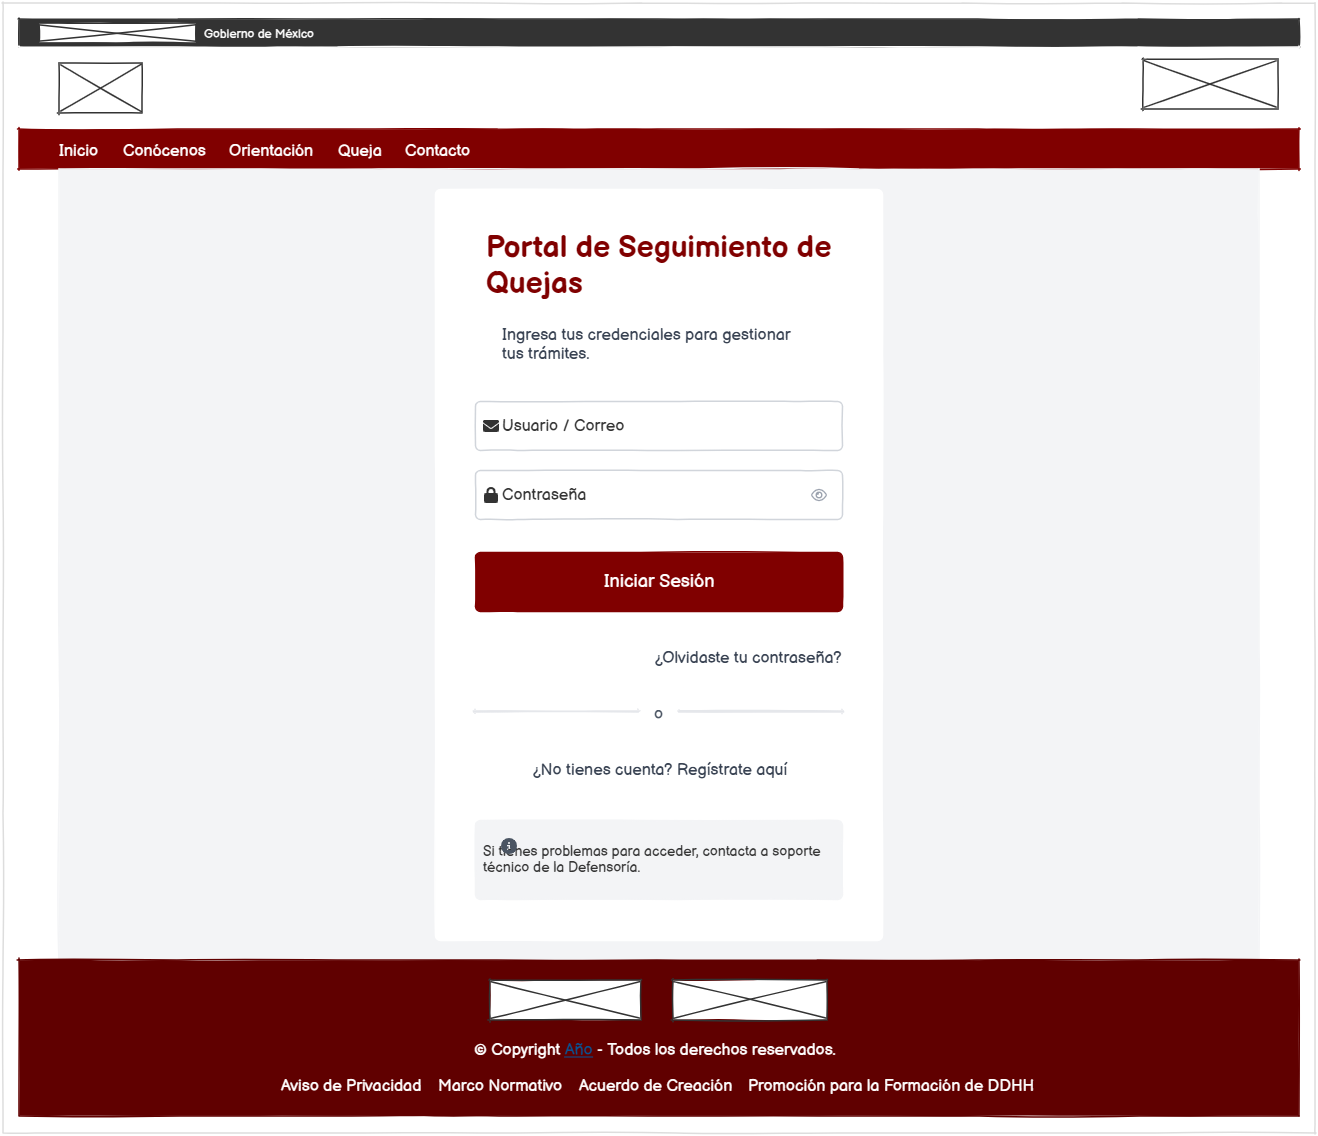
\includegraphics[width=0.80\textwidth, height=0.70\textheight, keepaspectratio]{imagenes/quejoso/Mockups/MQ-07_InicioSesionQuejoso.png}
    \caption{Mockup MQ-07: Pantalla de Inicio de Sesión}
    \label{fig:mq07_inicio_sesion}
\end{figure}

% ---- MQ-08 ----
\subsubsection{MQ-08: Opciones de Cuenta}

Pantalla de decisión que asiste al usuario que no cuenta con acceso. Ofrece dos rutas claras: iniciar el registro de una nueva queja desde cero o activar una cuenta de seguimiento utilizando un folio que ya le fue asignado previamente.

\begin{figure}[H]
    \centering
    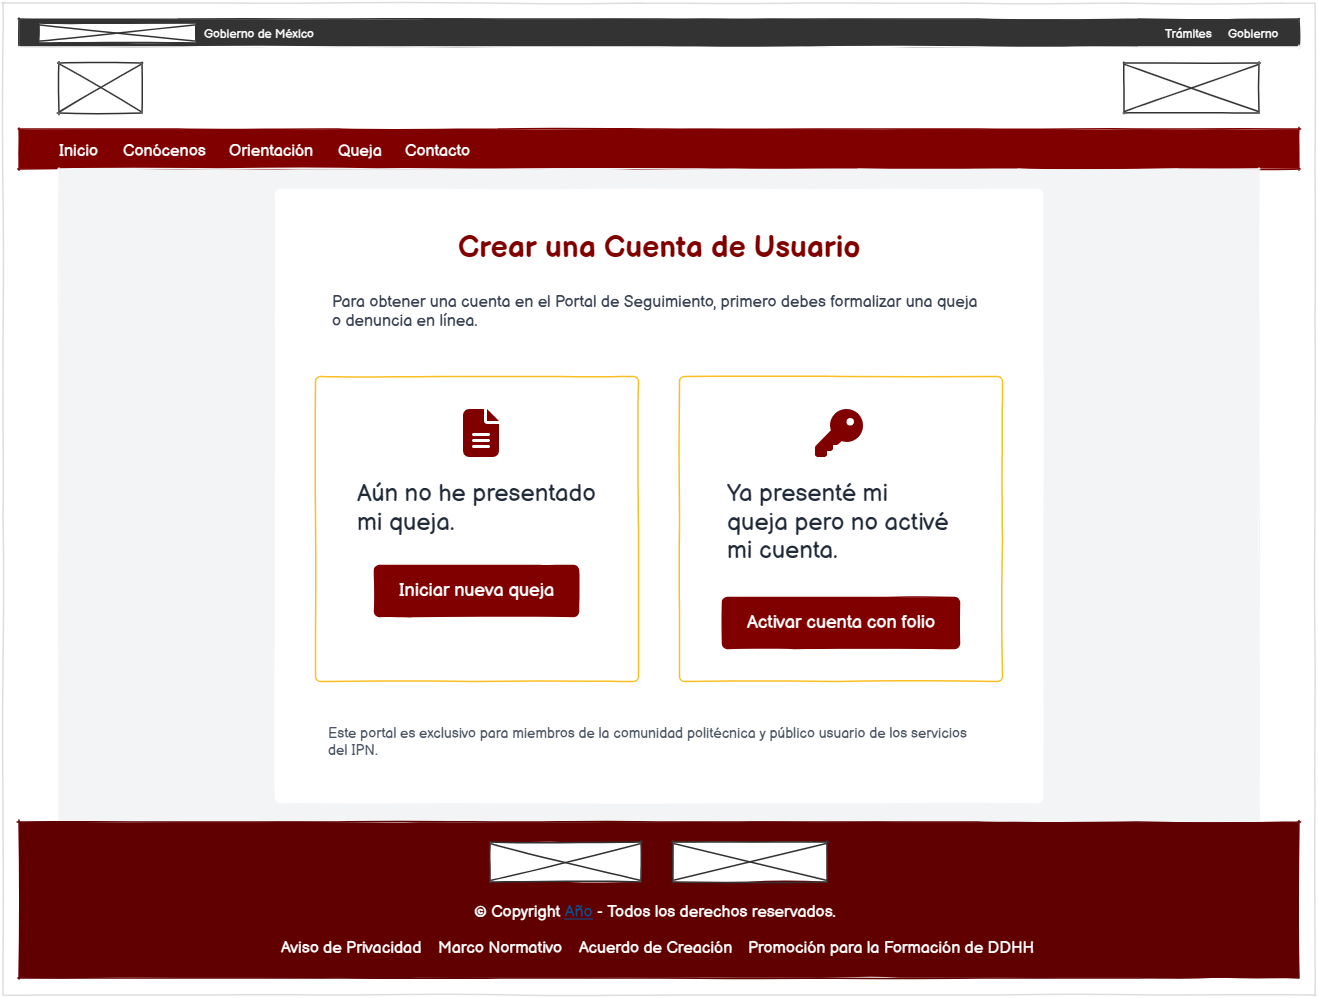
\includegraphics[width=0.80\textwidth, height=0.70\textheight, keepaspectratio]{imagenes/quejoso/Mockups/MQ-08_OpcionesCuenta.png}
    \caption{Mockup MQ-08: Opciones de Activación de Cuenta}
    \label{fig:mq08_opciones_cuenta}
\end{figure}

% ---- MQ-09 ----
\subsubsection{MQ-09: Cuenta Existente}

Interfaz de validación para usuarios que ya tienen un trámite en curso pero aún no han activado su perfil. Solicita el folio y el correo para verificar la identidad del solicitante en la base de datos antes de permitirle definir su contraseña de acceso.

\begin{figure}[H]
    \centering
    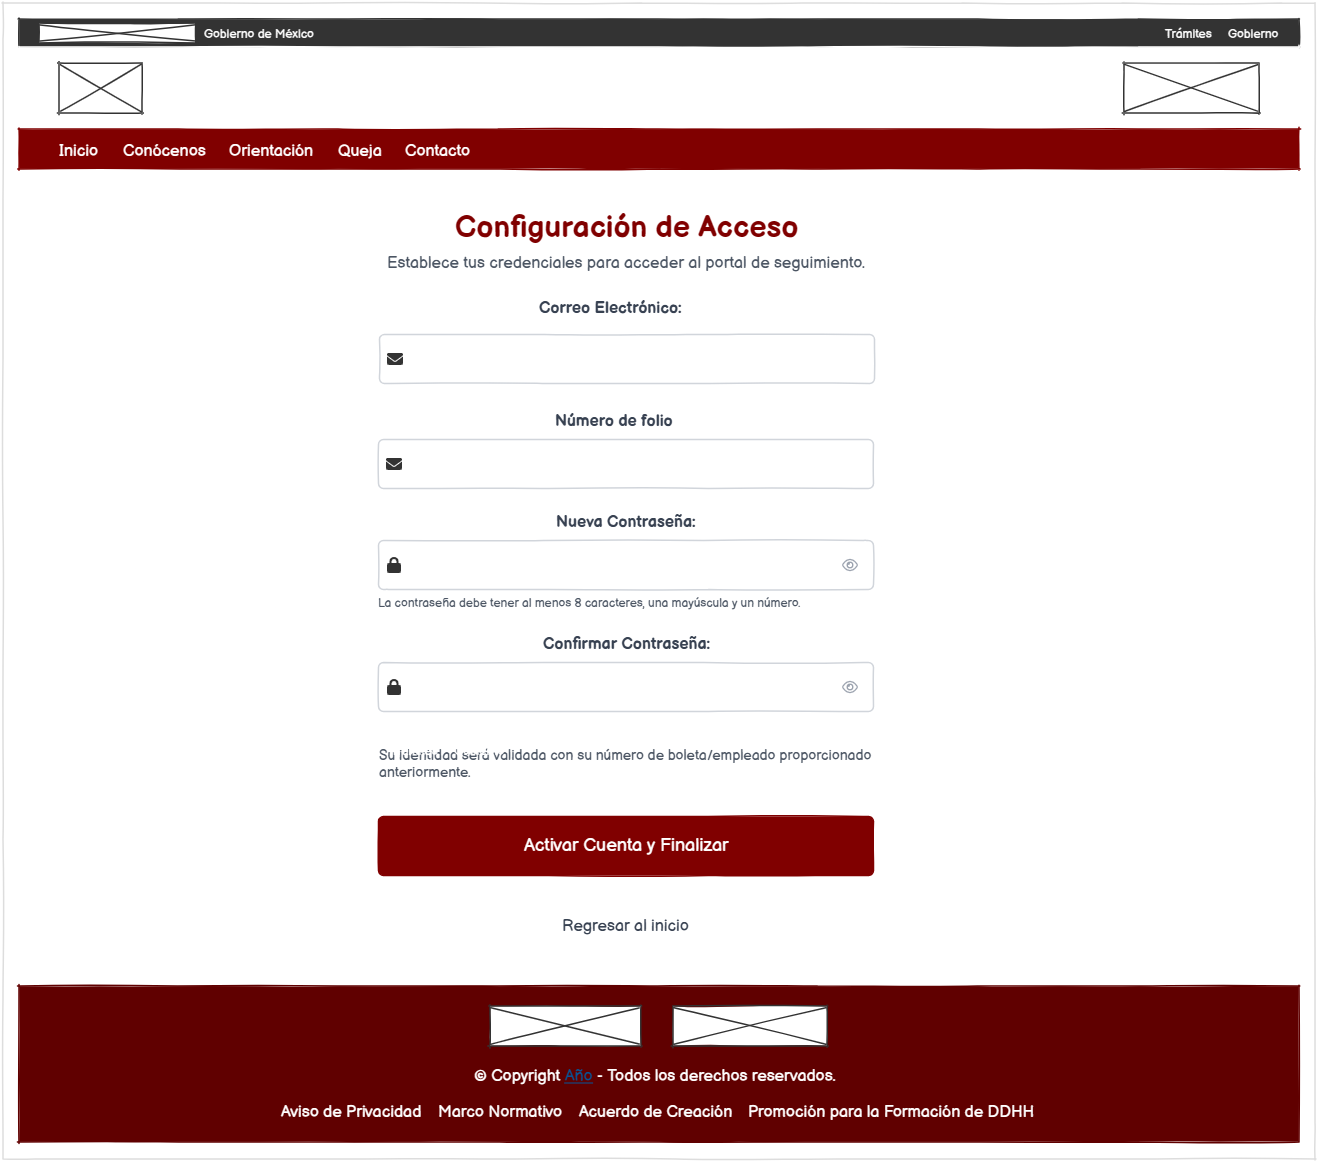
\includegraphics[width=0.80\textwidth, height=0.70\textheight, keepaspectratio]{imagenes/quejoso/Mockups/MQ-09_CuentaExistente.png}
    \caption{Mockup MQ-09: Aviso de Cuenta Existente}
    \label{fig:mq09_cuenta_existente}
\end{figure}

% ---- MQ-10 ----
\subsubsection{MQ-10: Restablecer Contraseña}

Flujo de recuperación de cuenta. Permite al usuario solicitar un enlace de restablecimiento mediante su correo electrónico registrado. Una vez validado el token, la interfaz habilita los campos para la creación y confirmación de la nueva credencial de acceso.

\begin{figure}[H]
    \centering
    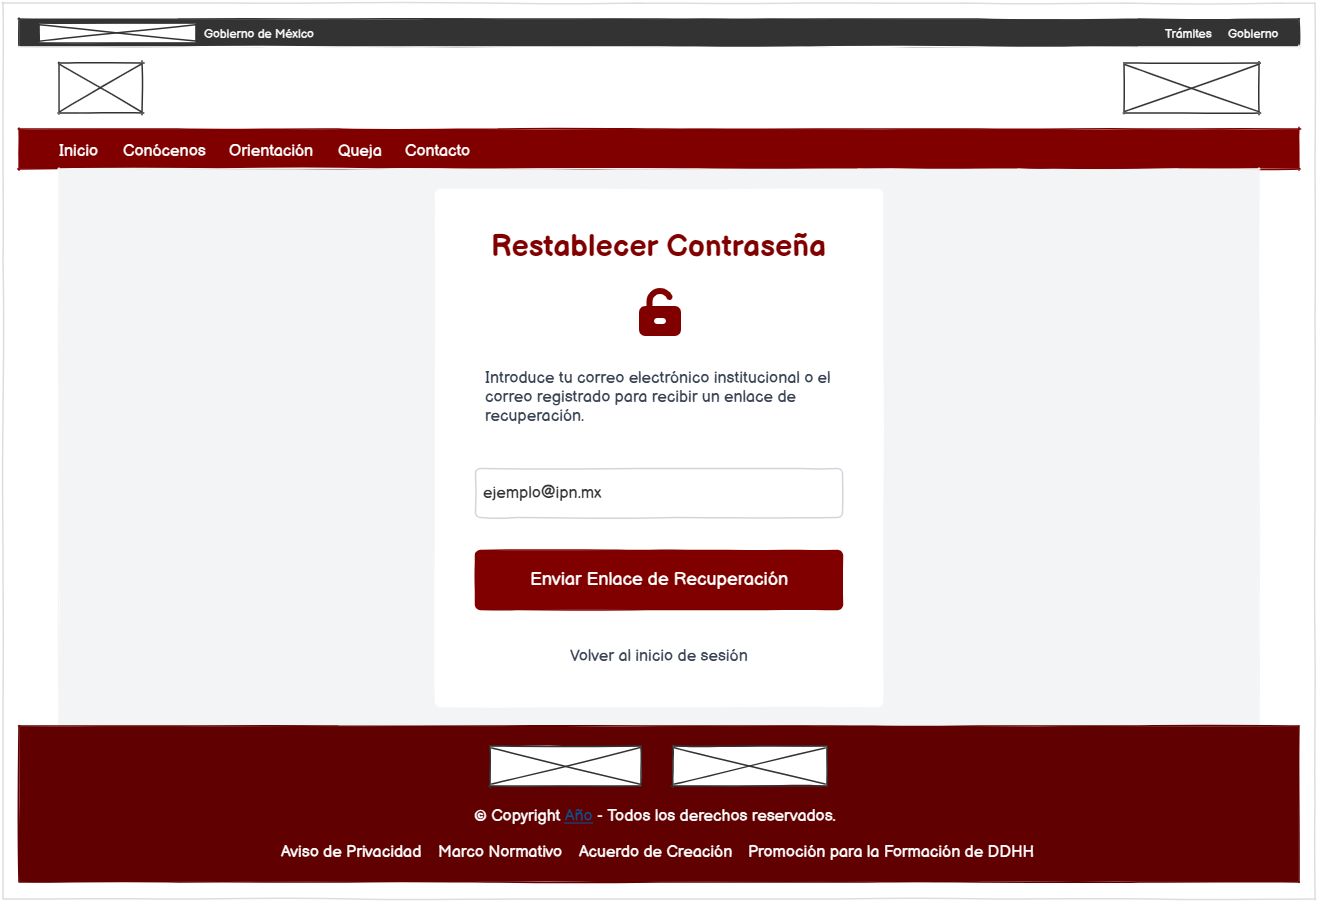
\includegraphics[width=0.80\textwidth, height=0.70\textheight, keepaspectratio]{imagenes/quejoso/Mockups/MQ-10_RestablecerPass.png}
    \caption{Mockup MQ-10: Pantalla de Restablecimiento de Contraseña}
    \label{fig:mq10_restablecer_pass}
\end{figure}

% ---- MQ-11 ----
\subsubsection{MQ-11: Gestión de Trámites (Dashboard)}

Representa la vista principal del usuario autenticado. Presenta un resumen ejecutivo con tarjetas de conteo estadístico sobre el estatus de sus quejas (Recibidas, En Revisión, Concluidas) y una tabla con los trámites más recientes, facilitando el acceso rápido a las acciones de edición, visualización o eliminación.

\begin{figure}[H]
    \centering
    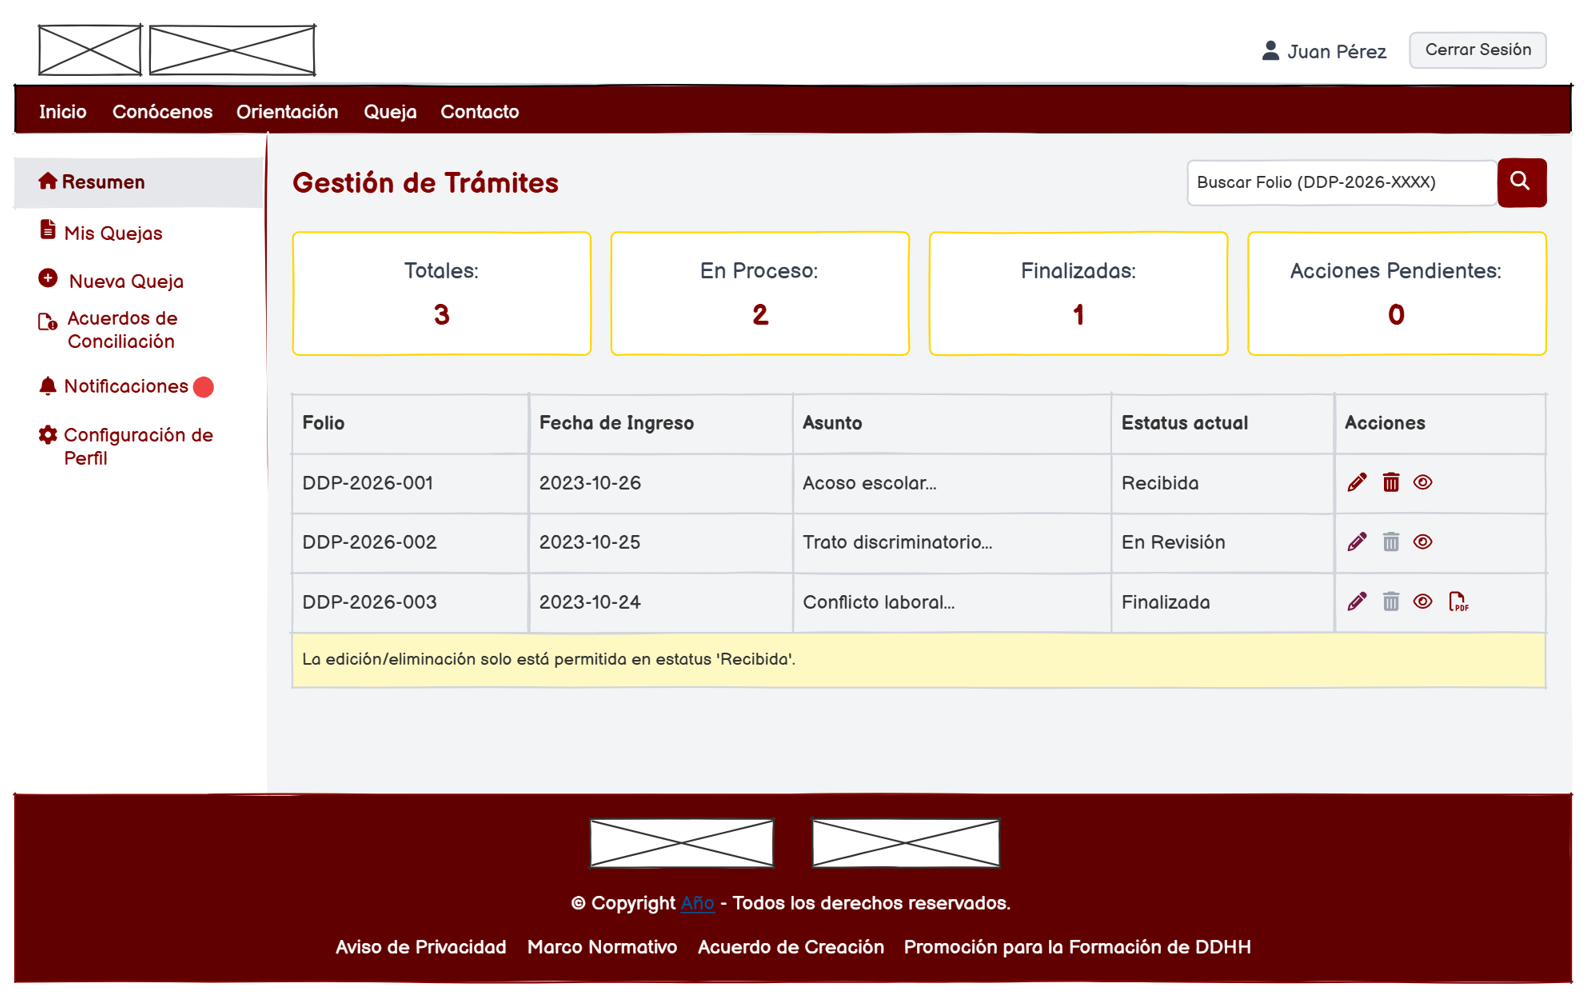
\includegraphics[width=0.80\textwidth, height=0.70\textheight, keepaspectratio]{imagenes/quejoso/Mockups/MQ-11_GestionTramites.png}
    \caption{Mockup MQ-11: Dashboard de Gestión de Trámites}
    \label{fig:mq11_gestion_tramites}
\end{figure}

% ---- MQ-12 ----
\subsubsection{MQ-12: Confirmar Eliminación}

Interfaz de diálogo modal diseñada para la eliminacion de una queja. Antes de procesar la cancelación lógica de un expediente, el sistema presenta una advertencia de seguridad para evitar eliminaciones accidentales. Esta opción solo se habilita si la queja se encuentra estrictamente en estatus "RECIBIDA".

\begin{figure}[H]
    \centering
    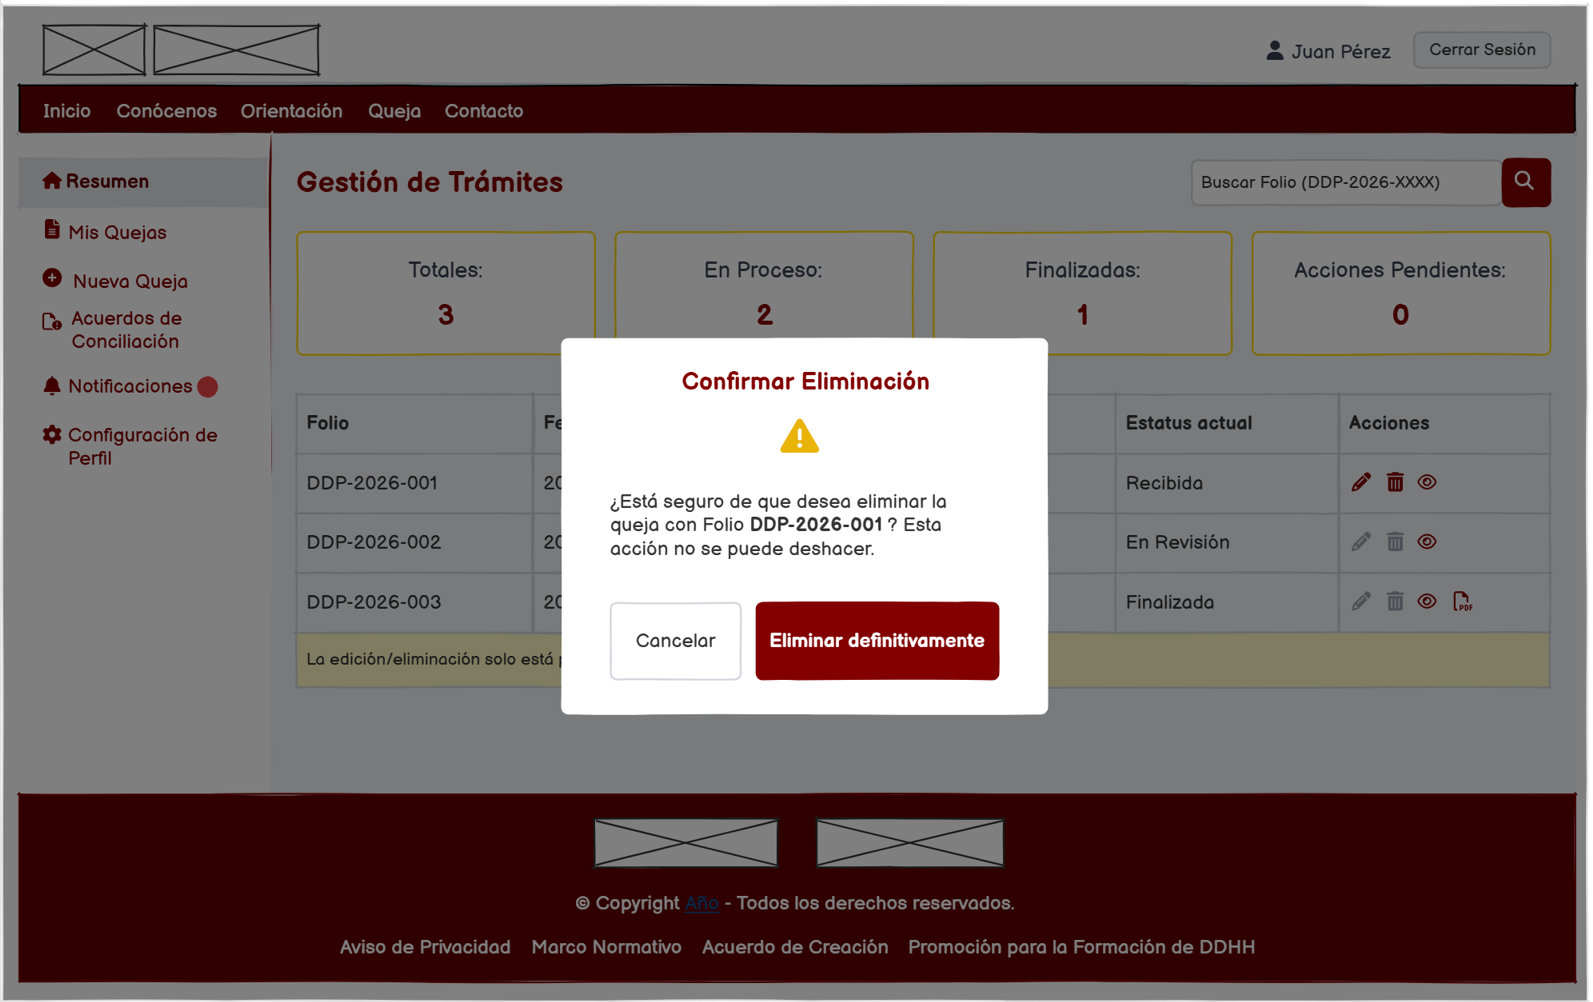
\includegraphics[width=0.80\textwidth, height=0.70\textheight, keepaspectratio]{imagenes/quejoso/Mockups/MQ-12_ConfirmarEliminacion.png}
    \caption{Mockup MQ-12: Diálogo de Confirmación de Eliminación}
    \label{fig:mq12_confirmar_eliminacion}
\end{figure}

% ---- MQ-13 ----
\subsubsection{MQ-13: Editar Queja}

Pantalla que permite al quejoso actualizar la información de su expediente. La interfaz carga los datos previamente registrados en el formulario, permitiendo modificar la narrativa de los hechos y gestionar los archivos de evidencia.

\begin{figure}[H]
    \centering
    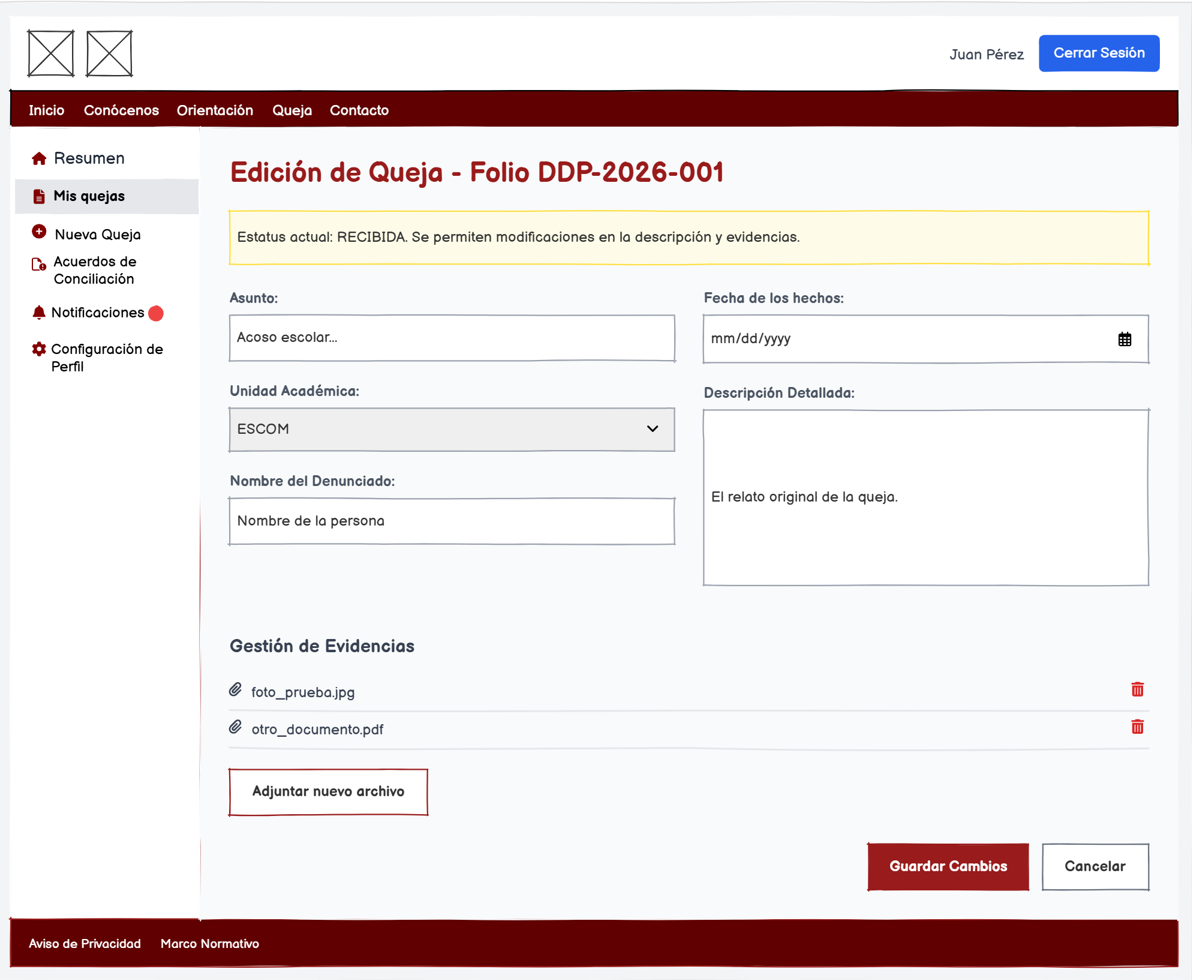
\includegraphics[width=0.80\textwidth, height=0.70\textheight, keepaspectratio]{imagenes/quejoso/Mockups/MQ-13_EditarQueja.png}
    \caption{Mockup MQ-13: Vista de Edición de Queja}
    \label{fig:mq13_editar_queja}
\end{figure}

% ---- MQ-14 ----
\subsubsection{MQ-14: Ver Detalles de Queja}

Interfaz de consulta de detalles de una queja. Despliega la información almacenada en un folio específico: datos del solicitante, cronología de estatus, narrativa de la queja y el repositorio de archivos adjuntos. Es una vista de solo lectura cuando el trámite ha avanzado a revisión.

\begin{figure}[H]
    \centering
    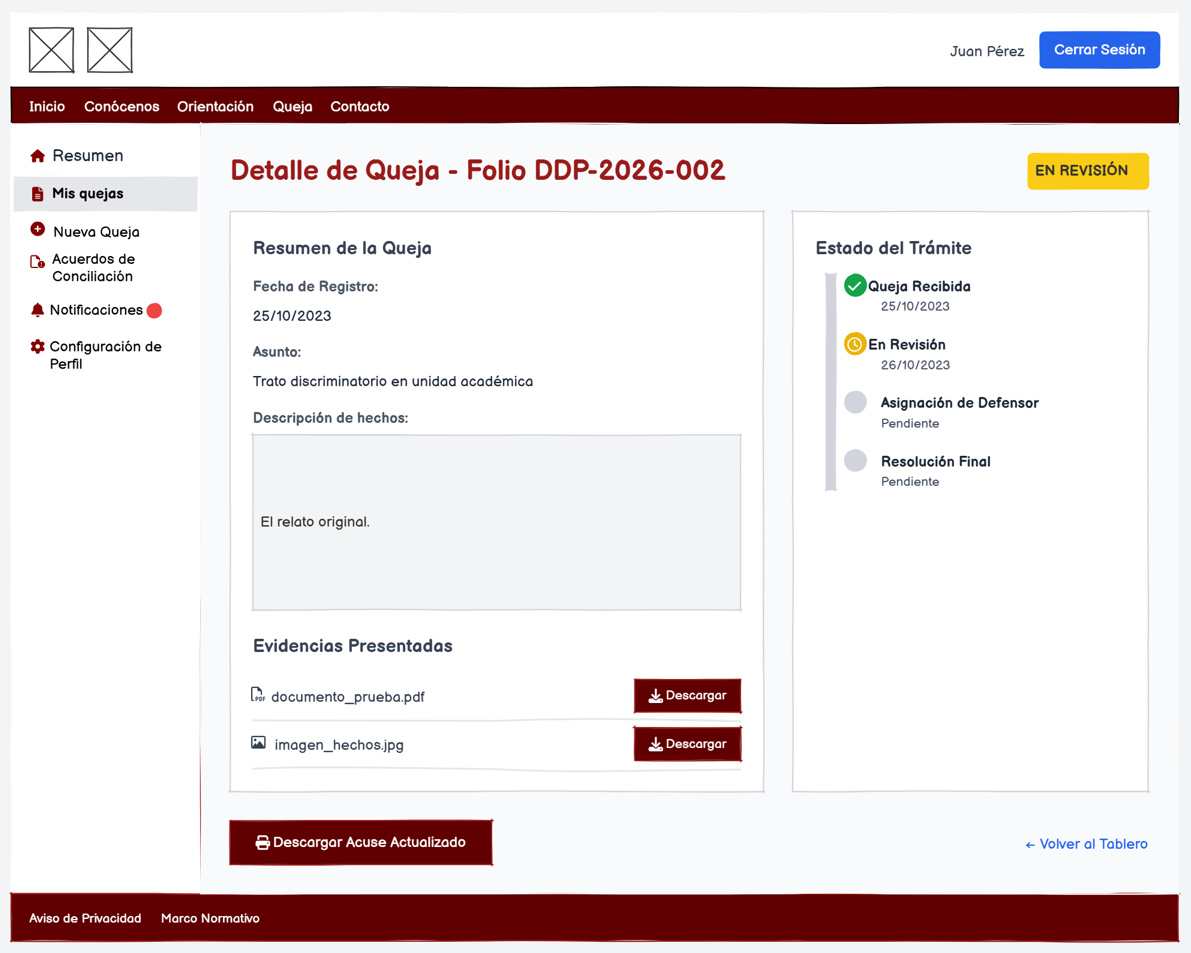
\includegraphics[width=0.80\textwidth, height=0.70\textheight, keepaspectratio]{imagenes/quejoso/Mockups/MQ-14_VerQueja.png}
    \caption{Mockup MQ-14: Vista de Detalle de Queja}
    \label{fig:mq14_ver_queja}
\end{figure}

% ---- MQ-15 ----
\subsubsection{MQ-15: Historial de Quejas}

Sección dedicada al un historial que presenta una tabla completa con todos los folios asociados al usuario. Incluye herramientas de filtrado avanzado por estatus y fecha, permitiendo al quejoso localizar expedientes históricos y descargar sus respectivos acuses de recibo.

\begin{figure}[H]
    \centering
    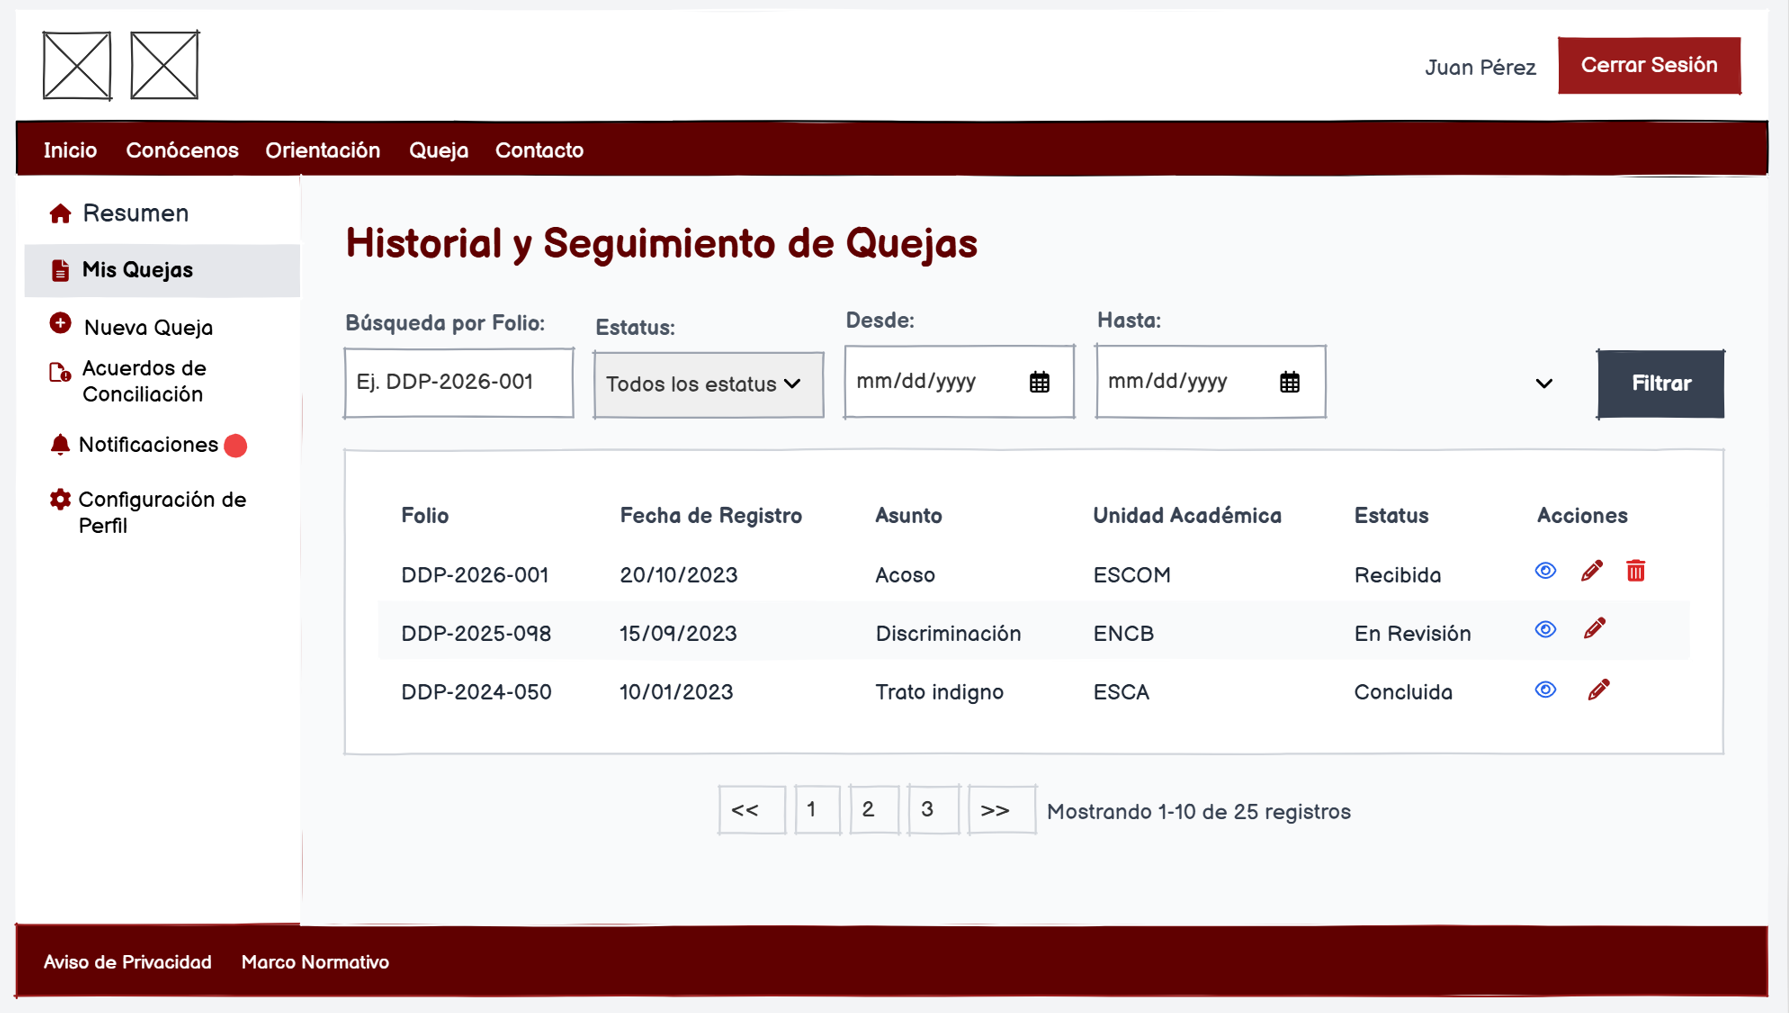
\includegraphics[width=0.80\textwidth, height=0.70\textheight, keepaspectratio]{imagenes/quejoso/Mockups/MQ-15_HistorialQuejas.png}
    \caption{Mockup MQ-15: Historial de Quejas del Usuario}
    \label{fig:mq15_historial_quejas}
\end{figure}

% ---- MQ-16 ----
\subsubsection{MQ-16: Nueva Queja (Autenticado)}

Formulario optimizado para levantar una nueva queja. A diferencia del registro público, esta interfaz recupera automáticamente los datos de perfil del usuario (nombre, correo, teléfono), permitiendo que el quejoso se enfoque únicamente en describir los nuevos hechos y adjuntar las evidencias correspondientes.

\begin{figure}[H]
    \centering
    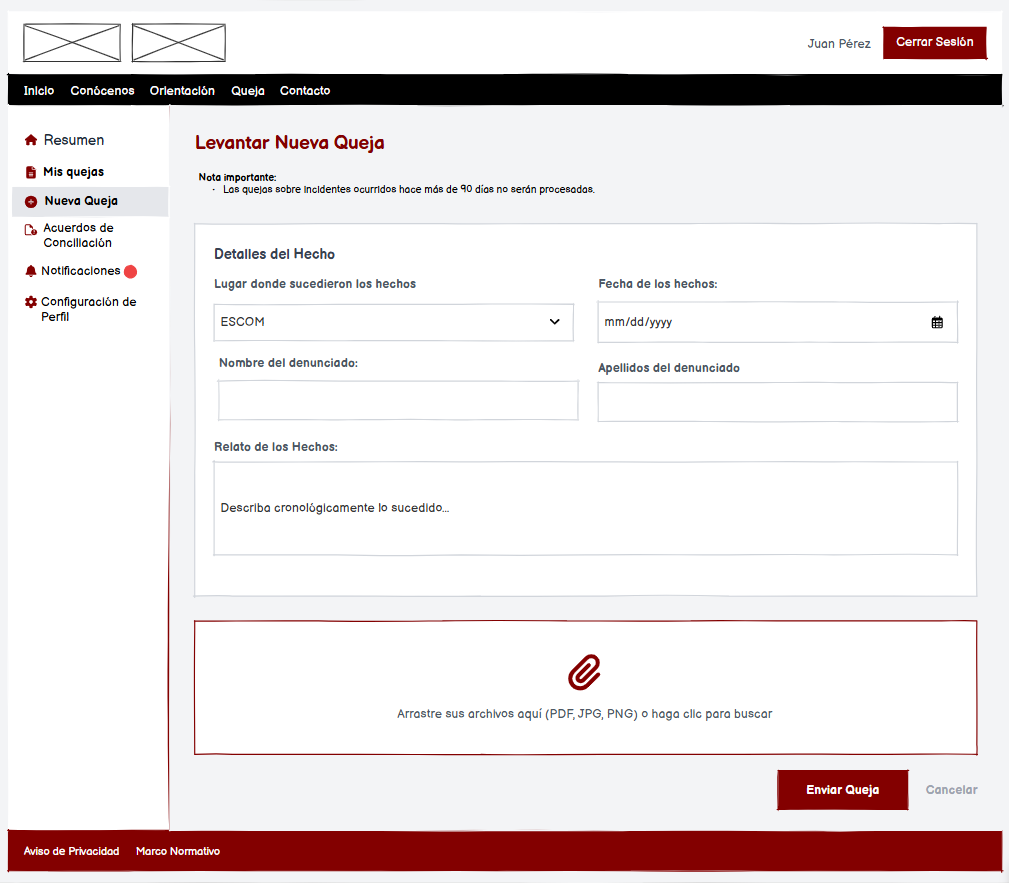
\includegraphics[width=0.80\textwidth, height=0.70\textheight, keepaspectratio]{imagenes/quejoso/Mockups/MQ-16_NuevaQueja.png}
    \caption{Mockup MQ-16: Formulario de Nueva Queja (Usuario Autenticado)}
    \label{fig:mq16_nueva_queja}
\end{figure}

% ---- MQ-17 ----
\subsubsection{MQ-17: Folio de Cuenta}

Vista de éxito tras registrar una nueva queja estando autenticado. Muestra el nuevo folio asignado y permite regresar de manera inmediata a la gestión de trámites, asegurando que el nuevo expediente aparezca actualizado en el historial del usuario.

\begin{figure}[H]
    \centering
    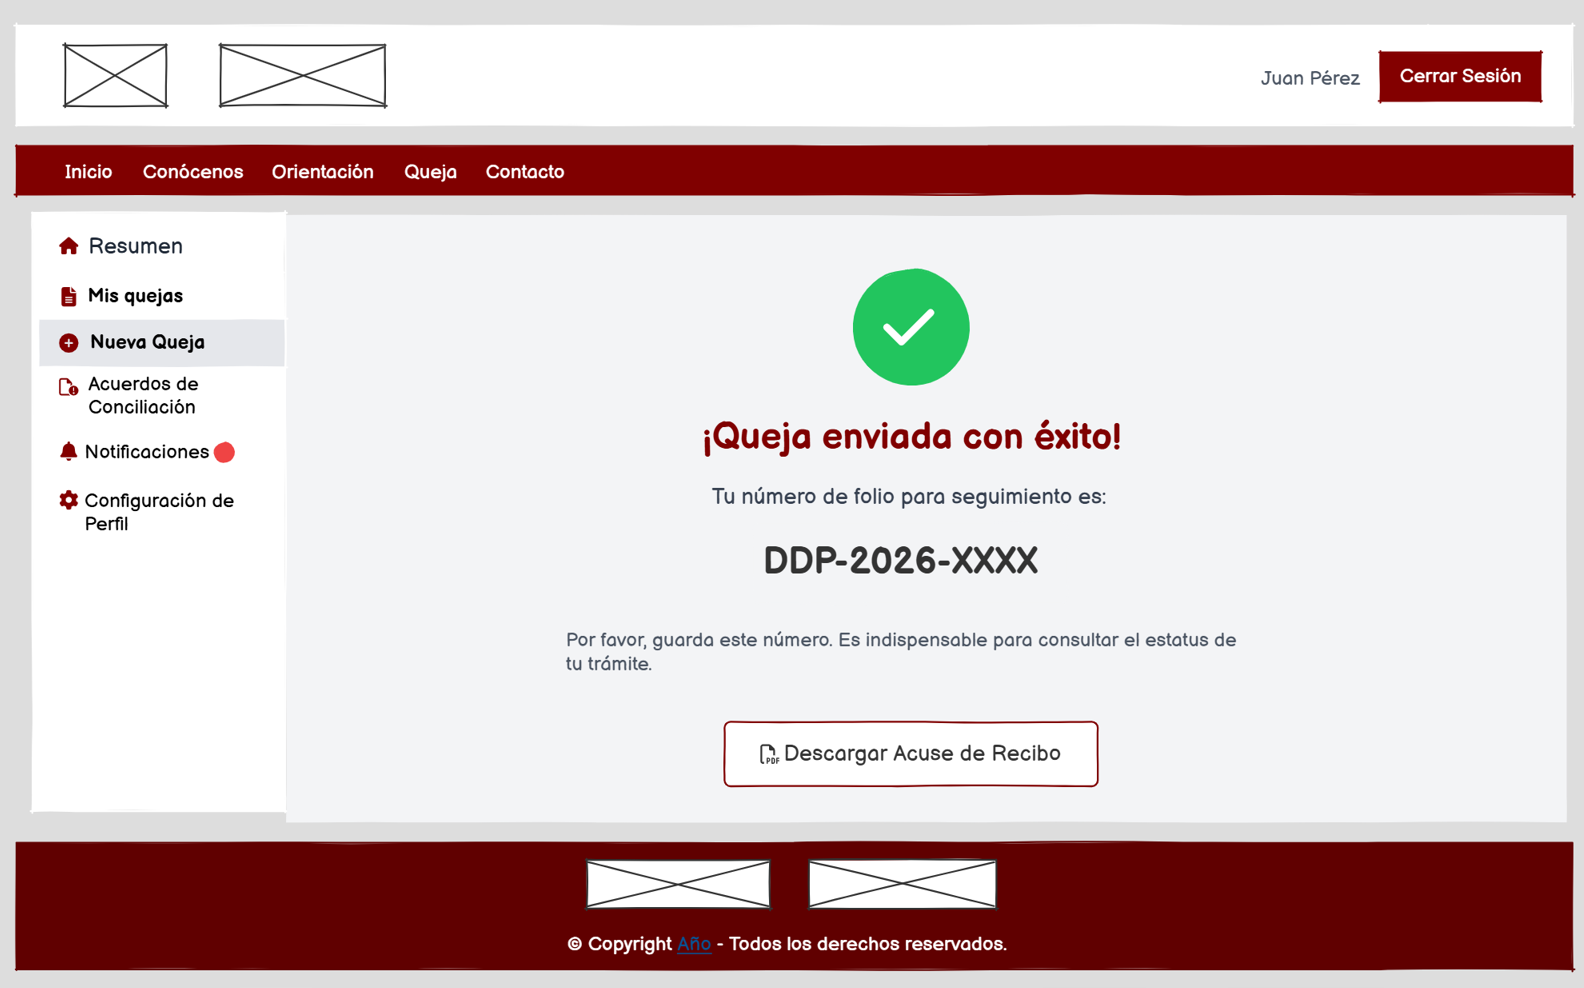
\includegraphics[width=0.80\textwidth, height=0.70\textheight, keepaspectratio]{imagenes/quejoso/Mockups/MQ-17_FolioCuenta.png}
    \caption{Mockup MQ-17: Confirmación de Folio en Cuenta Autenticada}
    \label{fig:mq17_folio_cuenta}
\end{figure}

% ---- MQ-18 ----
\subsubsection{MQ-18: Acuerdos de Conciliación}

Vista que agrupa los expedientes que han recibido una respuesta por parte del defensor. Permite al usuario identificar rápidamente cuáles de sus trámites tienen una propuesta pendiente de revisión, facilitando la transición hacia la resolución del conflicto.

\begin{figure}[H]
    \centering
    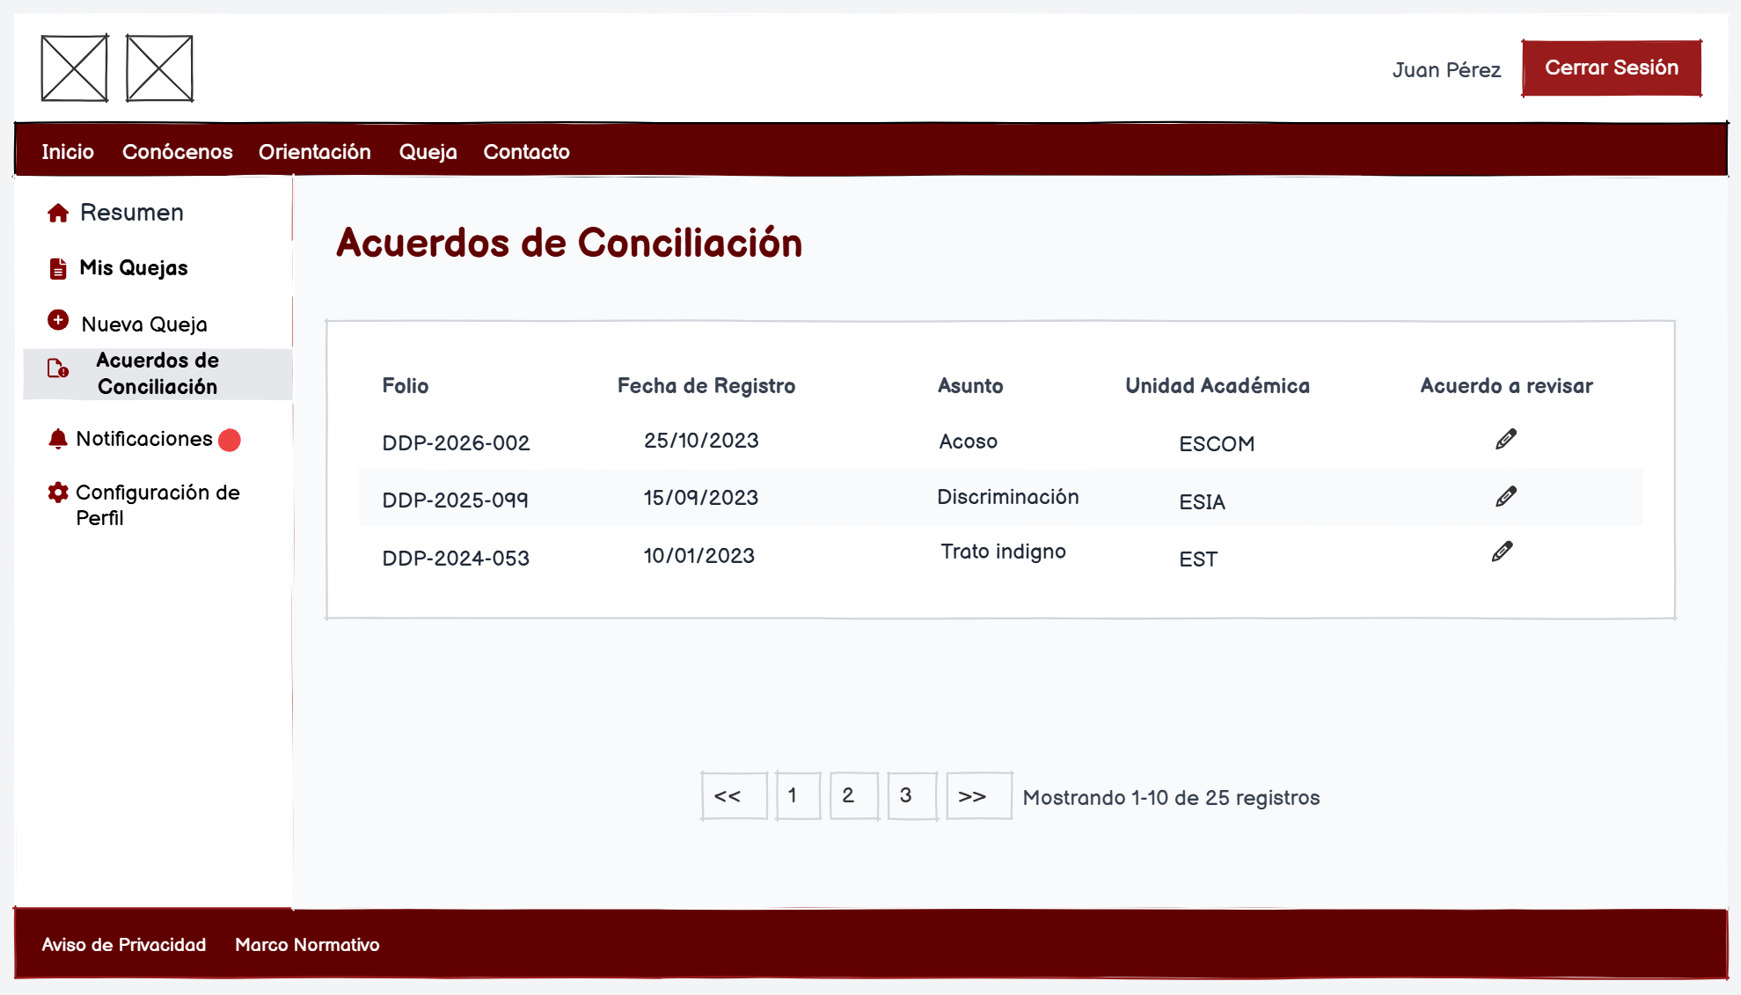
\includegraphics[width=0.80\textwidth, height=0.70\textheight, keepaspectratio]{imagenes/quejoso/Mockups/MQ-18_AcuerdosConciliacion.png}
    \caption{Mockup MQ-18: Vista de Acuerdos de Conciliación}
    \label{fig:mq18_acuerdos_conciliacion}
\end{figure}

% ---- MQ-19 ----
\subsubsection{MQ-19: Propuesta de Conciliación}

Pantalla para los procesos el proceso de aceptar o rechazar un acuerdo de conciliación. Presenta el texto de la solución propuesta por la Defensoría y habilita los controles vinculantes para que el quejoso pueda "Aceptar" o "Rechazar" la propuesta. En caso de rechazo, la interfaz solicita la justificación obligatoria.

\begin{figure}[H]
    \centering
    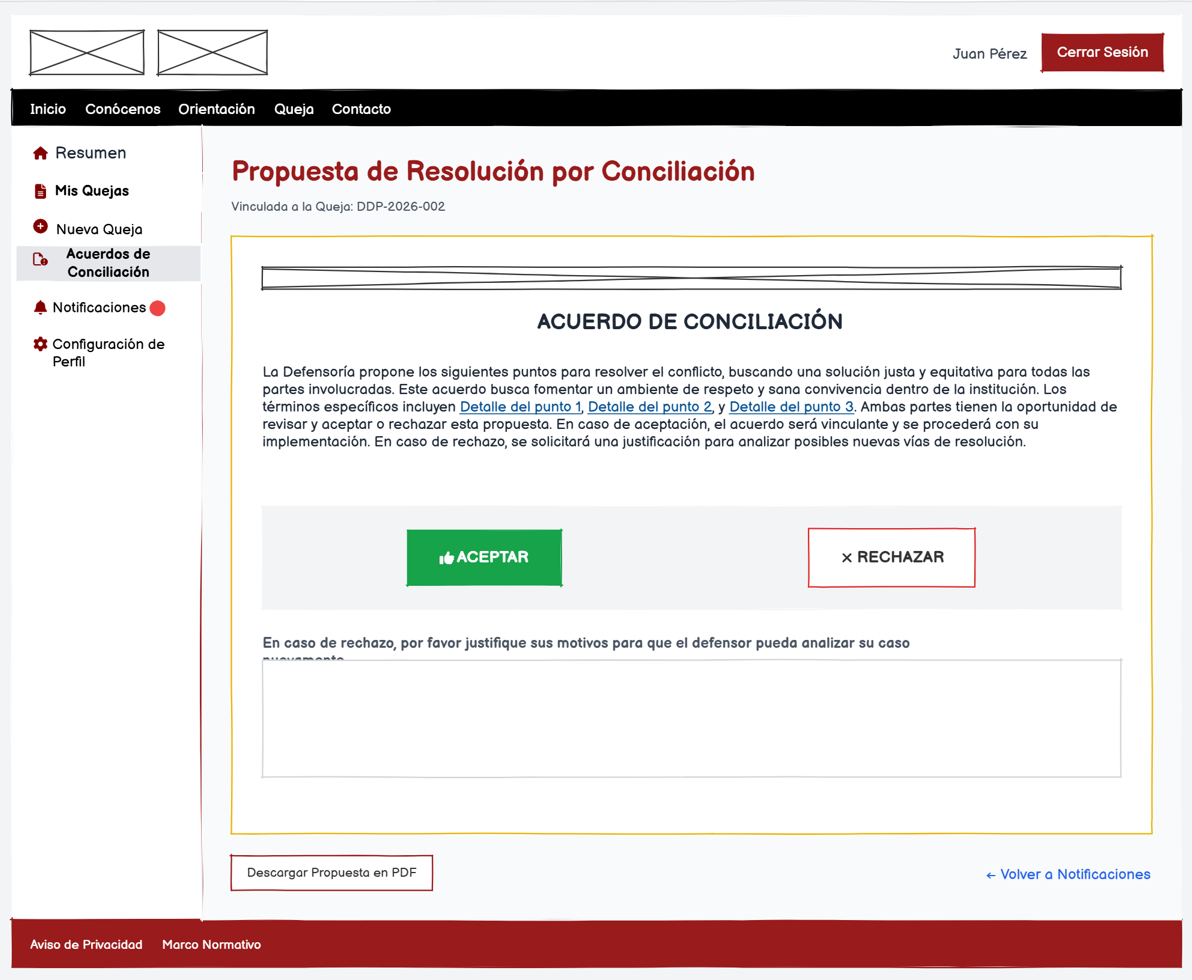
\includegraphics[width=0.80\textwidth, height=0.70\textheight, keepaspectratio]{imagenes/quejoso/Mockups/MQ-19_PropuestaConciliacion.png}
    \caption{Mockup MQ-19: Detalle de Propuesta de Conciliación}
    \label{fig:mq19_propuesta_conciliacion}
\end{figure}

% ---- MQ-20 ----
\subsubsection{MQ-20: Notificaciones}

Interfaz de alertas diseñada para mostrar una lista cronológica de eventos relevantes, como cambios de estatus en los expedientes o requerimientos de información adicional, permitiendo al quejoso mantenerse actualizado sobre el progreso administrativo de sus quejas.

\begin{figure}[H]
    \centering
    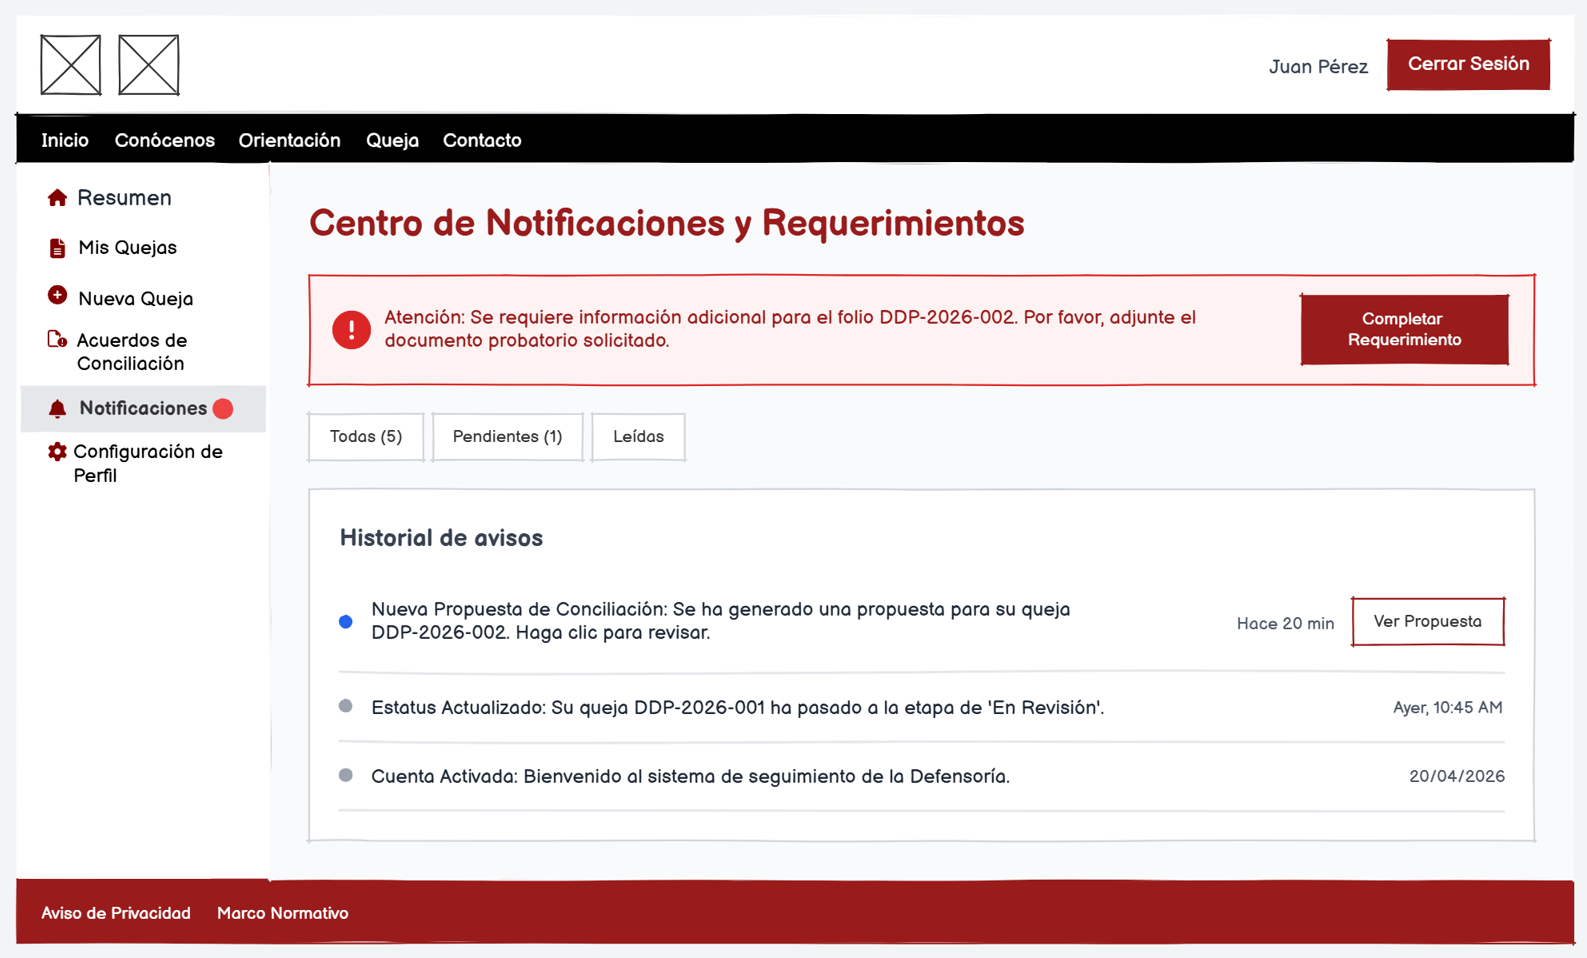
\includegraphics[width=0.80\textwidth, height=0.70\textheight, keepaspectratio]{imagenes/quejoso/Mockups/MQ-20_Notificaciones.png}
    \caption{Mockup MQ-20: Centro de Notificaciones}
    \label{fig:mq20_notificaciones}
\end{figure}

% ---- MQ-21 ----
\subsubsection{MQ-21: Configuración de Perfil}

Vista de perfil del quejoso autenticado. Muestra la información personal registrada en el sistema —nombre, correo, teléfono y datos del tutor si aplica— y permite editar los datos de contacto para mantenerlos actualizados durante el proceso de atención.

\begin{figure}[H]
    \centering
    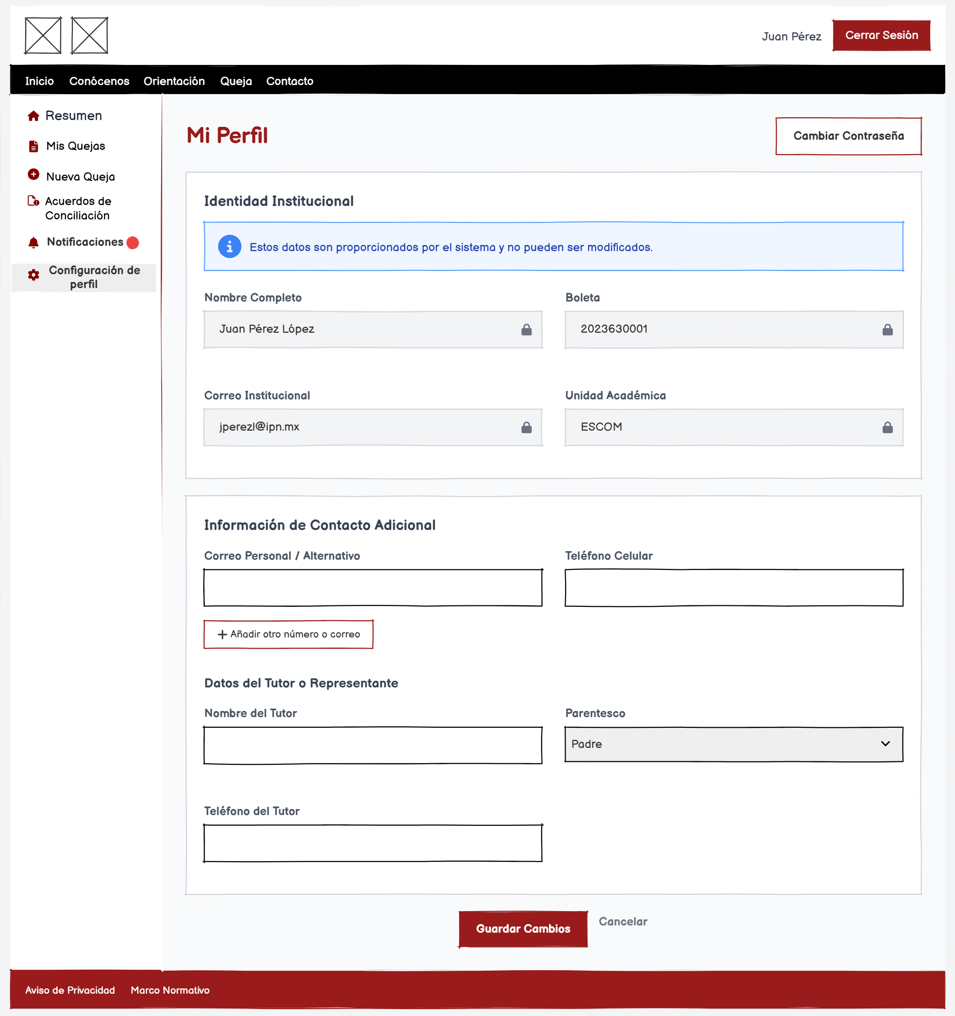
\includegraphics[width=0.80\textwidth, height=0.70\textheight, keepaspectratio]{imagenes/quejoso/Mockups/MQ-21_ConfiguracionPerfil.png}
    \caption{Mockup MQ-21: Configuración de Perfil del Quejoso}
    \label{fig:mq21_configuracion_perfil}
\end{figure}
